\documentclass[a4paper]{article}
\renewcommand{\epsilon}{\varepsilon}
\newcommand{\triposcourse}{Analysis and Topology}
\usepackage{fancyhdr,titlesec,geometry}
\usepackage[dvipsnames]{xcolor}
\usepackage[many]{tcolorbox}
\usepackage{xifthen}
\usepackage{import}
\usepackage{parskip}
\usepackage{transparent}
\usepackage{mathtools,amssymb,amsfonts,amsthm,bm}   % Math Presets
\usepackage{array,tabularx,booktabs}                % Table Presets
\usepackage{graphicx,wrapfig,float,caption}         % Figure Presets
\usepackage{setspace,multicol}                      % Text Presets
\usepackage{tikz,physics,cancel,tkz-euclide,pgfplots,tikz-3dplot}                    % Physics Presets
\usepackage{amsmath}
\usepackage{mathrsfs}
\usepackage{enumerate}
\usepackage[shortlabels]{enumitem}
\usepackage{hyperref}
\usepackage{lipsum}
\usepackage{IEEEtrantools}
\usepackage{xcomment}
\usepackage{sectsty}
\usepackage{thmtools}
\usepackage{mdframed}
\usepackage{siunitx}
\usepackage{centernot}

\newcommand{\sectionbreak}{\clearpage}

\tdplotsetmaincoords{60}{120}

\usetikzlibrary{arrows.meta}
\usetikzlibrary{decorations.markings}
\usetikzlibrary{decorations.pathmorphing}
\usetikzlibrary{automata, positioning}
\usetikzlibrary{fadings}
\usetikzlibrary{intersections}
\usetikzlibrary{cd}
\usetikzlibrary{patterns}
\usetikzlibrary{shapes.arrows}
\usepgfplotslibrary{colormaps, external}
\pgfarrowsdeclarecombine{twolatex'}{twolatex'}{latex'}{latex'}{latex'}{latex'}
\tikzset{->/.style = {decoration={markings,
                                  mark=at position 1 with {\arrow[scale=1.6]{latex'}}},
                      postaction={decorate}}}
\tikzset{<-/.style = {decoration={markings,
                                  mark=at position 0 with {\arrowreversed[scale=1.6]{latex'}}},
                      postaction={decorate}}}
\tikzset{<->/.style = {decoration={markings,
                                   mark=at position 0 with {\arrowreversed[scale=1.6]{latex'}},
                                   mark=at position 1 with {\arrow[scale=1.6]{latex'}}},
                       postaction={decorate}}}
\tikzset{->-/.style = {decoration={markings,
                                   mark=at position #1 with {\arrow[scale=1.6]{latex'}}},
                       postaction={decorate}}}
\tikzset{-<-/.style = {decoration={markings,
                                   mark=at position #1 with {\arrowreversed[scale=1.6]{latex'}}},
                       postaction={decorate}}}
\tikzset{->>/.style = {decoration={markings,
                                  mark=at position 1 with {\arrow[scale=1.6]{twolatex'}}},
                      postaction={decorate}}}
\tikzset{<<-/.style = {decoration={markings,
                                  mark=at position 0 with {\arrowreversed[scale=1.6]{twolatex'}}},
                      postaction={decorate}}}
\tikzset{<<->>/.style = {decoration={markings,
                                   mark=at position 0 with {\arrowreversed[scale=1.6]{twolatex'}},
                                   mark=at position 1 with {\arrow[scale=1.6]{twolatex'}}},
                       postaction={decorate}}}
\tikzset{->>-/.style = {decoration={markings,
                                   mark=at position #1 with {\arrow[scale=1.6]{twolatex'}}},
                       postaction={decorate}}}
\tikzset{-<<-/.style = {decoration={markings,
                                   mark=at position #1 with {\arrowreversed[scale=1.6]{twolatex'}}},
                       postaction={decorate}}}

\tikzset{
set arrow inside/.code={\pgfqkeys{/tikz/arrow inside}{#1}},
set arrow inside={end/.initial=>, opt/.initial=},
/pgf/decoration/Mark/.style={
    mark/.expanded=at position #1 with
    {
        \noexpand\arrow[\pgfkeysvalueof{/tikz/arrow inside/opt}]{\pgfkeysvalueof{/tikz/arrow inside/end}}
    }
},
arrow inside/.style 2 args={
    set arrow inside={#1},
    postaction={
        decorate,decoration={
            markings,Mark/.list={#2}
        }
    }
},
}

\tikzstyle{circ}=[fill=black, draw=black, shape=circle]
\tikzset{
dot/.style = {circle, fill, minimum size=#1,
              inner sep=0pt, outer sep=0pt},
dot/.default = 5pt% size of the circle diameter 
}
\tikzset{mstate/.style={circle, draw, blue, text=black, minimum width=0.7cm}}
\tikzset{snake it/.style={-stealth,
decoration={snake, 
    amplitude = .4mm,
    segment length = 2mm,
    post length=0.9mm},decorate}}

\def\centerarc[#1](#2)(#3:#4:#5)% Syntax: [draw options](center)(initial angle:final angle:radius)
    { \draw[#1] ($(#2)+({#5*cos(#3)},{#5*sin(#3)})$) arc (#3:#4:#5); }

\hypersetup{
    colorlinks=true,
    linkcolor=blue,
    filecolor=blue,
    citecolor = black,      
    urlcolor=cyan,
    }

%%%%%%%%%%% Snippets %%%%%%%%%%%%%%%%
\newcommand*\widefbox[1]{\fbox{\hspace{2em}#1\hspace{2em}}}
\newcommand{\xint}{\int_{x_1}^{x_2}}
\newcommand{\mw}{\sqrt{m\omega}}
\newcommand{\de}{\delta}
\newcommand{\dde}{\dot{\delta}}
\newcommand{\di}{\delta_i}
\newcommand{\ddi}{\dot{\delta_i}}
\newcommand{\dddi}{\ddot{\delta_i}}
\newcommand{\dipl}{\delta_{i+1}}
\newcommand{\dimi}{\delta_{i-1}}
\newcommand{\ddt}[1]{\frac{{d} #1}{dt}}
\newcommand{\ddtt}[1]{\frac{d^2 #1}{dt^2}}
\newcommand{\ddx}[1]{\frac{d #1}{dx}}
\newcommand{\ddxx}[1]{\frac{d^2 #1}{dx^2}}
\newcommand{\eps}{\epsilon}
\newcommand{\del}[2]{\frac{\partial #1}{\partial #2}}
\newcommand{\deltwo}[2]{\frac{\partial^2 #1}{\partial #2^2}}
\newcommand{\lam}{\lambda}
\newcommand{\Lam}{\Lambda}
\newcommand{\sig}{\sigma}
\newcommand{\Sig}{\Sigma}
\newcommand{\half}{\frac{1}{2}}
\newcommand{\munu}{{\mu\nu}}
\newcommand{\thalf}{\tfrac{1}{2}}
\renewcommand{\div}{\nabla\cdot}
\renewcommand{\curl}{\nabla\times}

\DeclareMathOperator{\orb}{Orb}
\DeclareMathOperator{\stab}{Stab}
\DeclareMathOperator{\adj}{adj}
\DeclareMathOperator{\ccl}{ccl}
\let\var\relax
\DeclareMathOperator{\var}{Var}
\DeclareMathOperator{\cov}{Cov}
\DeclareMathOperator{\corr}{Corr}
\DeclareMathOperator{\Markov}{Markov}
\DeclareMathOperator{\nullity}{nullity}

\newcommand{\bfA}{{\bf A}}
\newcommand{\bfB}{{\bf B}}
\newcommand{\bfC}{{\bf C}}
\newcommand{\bfD}{{\bf D}}
\newcommand{\bfE}{{\bf E}}
\newcommand{\bfF}{{\bf F}}
\newcommand{\bfG}{{\bf G}}
\newcommand{\bfH}{{\bf H}}
\newcommand{\bfI}{{\bf I}}
\newcommand{\bfJ}{{\bf J}}
\newcommand{\bfK}{{\bf K}}
\newcommand{\bfL}{{\bf L}}
\newcommand{\bfM}{{\bf M}}
\newcommand{\bfN}{{\bf N}}
\newcommand{\bfO}{{\bf O}}
\newcommand{\bfP}{{\bf P}}
\newcommand{\bfQ}{{\bf Q}}
\newcommand{\bfR}{{\bf R}}
\newcommand{\bfS}{{\bf S}}
\newcommand{\bfT}{{\bf T}}
\newcommand{\bfU}{{\bf U}}
\newcommand{\bfV}{{\bf V}}
\newcommand{\bfW}{{\bf W}}
\newcommand{\bfX}{{\bf X}}
\newcommand{\bfY}{{\bf Y}}
\newcommand{\bfZ}{{\bf Z}}

\newcommand{\bfa}{{\bf a}}
\newcommand{\bfb}{{\bf b}}
\newcommand{\bfc}{{\bf c}}
\newcommand{\bfd}{{\bf d}}
\newcommand{\bfe}{{\bf e}}
\newcommand{\bff}{{\bf f}}
\newcommand{\bfg}{{\bf g}}
\newcommand{\bfh}{{\bf h}}
\newcommand{\bfi}{{\bf i}}
\newcommand{\bfj}{{\bf j}}
\newcommand{\bfk}{{\bf k}}
\newcommand{\bfl}{{\bf l}}
\newcommand{\bfm}{{\bf m}}
\newcommand{\bfn}{{\bf n}}
\newcommand{\bfo}{{\bf o}}
\newcommand{\bfp}{{\bf p}}
\newcommand{\bfq}{{\bf q}}
\newcommand{\bfr}{{\bf r}}
\newcommand{\bfs}{{\bf s}}
\newcommand{\bft}{{\bf t}}
\newcommand{\bfu}{{\bf u}}
\newcommand{\bfv}{{\bf v}}
\newcommand{\bfw}{{\bf w}}
\newcommand{\bfx}{{\bf x}}
\newcommand{\bfy}{{\bf y}}
\newcommand{\bfz}{{\bf z}}

\newcommand{\mcA}{{\mathcal{A}}}
\newcommand{\mcB}{{\mathcal{B}}}
\newcommand{\mcC}{{\mathcal{C}}}
\newcommand{\mcD}{{\mathcal{D}}}
\newcommand{\mcE}{{\mathcal{E}}}
\newcommand{\mcF}{{\mathcal{F}}}
\newcommand{\mcG}{{\mathcal{G}}}
\newcommand{\mcH}{{\mathcal{H}}}
\newcommand{\mcI}{{\mathcal{I}}}
\newcommand{\mcJ}{{\mathcal{J}}}
\newcommand{\mcK}{{\mathcal{K}}}
\newcommand{\mcL}{{\mathcal{L}}}
\newcommand{\mcM}{{\mathcal{M}}}
\newcommand{\mcN}{{\mathcal{N}}}
\newcommand{\mcO}{{\mathcal{O}}}
\newcommand{\mcP}{{\mathcal{P}}}
\newcommand{\mcQ}{{\mathcal{Q}}}
\newcommand{\mcR}{{\mathcal{R}}}
\newcommand{\mcS}{{\mathcal{S}}}
\newcommand{\mcT}{{\mathcal{T}}}
\newcommand{\mcU}{{\mathcal{U}}}
\newcommand{\mcV}{{\mathcal{V}}}
\newcommand{\mcW}{{\mathcal{W}}}
\newcommand{\mcX}{{\mathcal{X}}}
\newcommand{\mcY}{{\mathcal{Y}}}
\newcommand{\mcZ}{{\mathcal{Z}}}

\newcommand{\bbA}{{\mathbb{A}}}
\newcommand{\bbB}{{\mathbb{B}}}
\newcommand{\bbC}{{\mathbb{C}}}
\newcommand{\bbD}{{\mathbb{D}}}
\newcommand{\bbE}{{\mathbb{E}}}
\newcommand{\bbF}{{\mathbb{F}}}
\newcommand{\bbG}{{\mathbb{G}}}
\newcommand{\bbH}{{\mathbb{H}}}
\newcommand{\bbI}{{\mathbb{I}}}
\newcommand{\bbJ}{{\mathbb{J}}}
\newcommand{\bbK}{{\mathbb{K}}}
\newcommand{\bbL}{{\mathbb{L}}}
\newcommand{\bbM}{{\mathbb{M}}}
\newcommand{\bbN}{{\mathbb{N}}}
\newcommand{\bbO}{{\mathbb{O}}}
\newcommand{\bbP}{{\mathbb{P}}}
\newcommand{\bbQ}{{\mathbb{Q}}}
\newcommand{\bbR}{{\mathbb{R}}}
\newcommand{\bbS}{{\mathbb{S}}}
\newcommand{\bbT}{{\mathbb{T}}}
\newcommand{\bbU}{{\mathbb{U}}}
\newcommand{\bbV}{{\mathbb{V}}}
\newcommand{\bbW}{{\mathbb{W}}}
\newcommand{\bbX}{{\mathbb{X}}}
\newcommand{\bbY}{{\mathbb{Y}}}
\newcommand{\bbZ}{{\mathbb{Z}}}

\newcommand{\mfa}{{\mathfrak{a}}}
\newcommand{\mfb}{{\mathfrak{b}}}
\newcommand{\mfc}{{\mathfrak{c}}}
\newcommand{\mfd}{{\mathfrak{d}}}
\newcommand{\mfe}{{\mathfrak{e}}}
\newcommand{\mff}{{\mathfrak{f}}}
\newcommand{\mfg}{{\mathfrak{g}}}
\newcommand{\mfh}{{\mathfrak{h}}}
\newcommand{\mfi}{{\mathfrak{i}}}
\newcommand{\mfj}{{\mathfrak{j}}}
\newcommand{\mfk}{{\mathfrak{k}}}
\newcommand{\mfl}{{\mathfrak{l}}}
\newcommand{\mfm}{{\mathfrak{m}}}
\newcommand{\mfn}{{\mathfrak{n}}}
\newcommand{\mfo}{{\mathfrak{o}}}
\newcommand{\mfp}{{\mathfrak{p}}}
\newcommand{\mfq}{{\mathfrak{q}}}
\newcommand{\mfr}{{\mathfrak{r}}}
\newcommand{\mfs}{{\mathfrak{s}}}
\newcommand{\mft}{{\mathfrak{t}}}
\newcommand{\mfu}{{\mathfrak{u}}}
\newcommand{\mfv}{{\mathfrak{v}}}
\newcommand{\mfw}{{\mathfrak{w}}}
\newcommand{\mfx}{{\mathfrak{x}}}
\newcommand{\mfy}{{\mathfrak{y}}}
\newcommand{\mfz}{{\mathfrak{z}}}

\newcommand{\mfA}{{\mathfrak{A}}}
\newcommand{\mfB}{{\mathfrak{B}}}
\newcommand{\mfC}{{\mathfrak{C}}}
\newcommand{\mfD}{{\mathfrak{D}}}
\newcommand{\mfE}{{\mathfrak{E}}}
\newcommand{\mfF}{{\mathfrak{F}}}
\newcommand{\mfG}{{\mathfrak{G}}}
\newcommand{\mfH}{{\mathfrak{H}}}
\newcommand{\mfI}{{\mathfrak{I}}}
\newcommand{\mfJ}{{\mathfrak{J}}}
\newcommand{\mfK}{{\mathfrak{K}}}
\newcommand{\mfL}{{\mathfrak{L}}}
\newcommand{\mfM}{{\mathfrak{M}}}
\newcommand{\mfN}{{\mathfrak{N}}}
\newcommand{\mfO}{{\mathfrak{O}}}
\newcommand{\mfP}{{\mathfrak{P}}}
\newcommand{\mfQ}{{\mathfrak{Q}}}
\newcommand{\mfR}{{\mathfrak{R}}}
\newcommand{\mfS}{{\mathfrak{S}}}
\newcommand{\mfT}{{\mathfrak{T}}}
\newcommand{\mfU}{{\mathfrak{U}}}
\newcommand{\mfV}{{\mathfrak{V}}}
\newcommand{\mfW}{{\mathfrak{W}}}
\newcommand{\mfX}{{\mathfrak{X}}}
\newcommand{\mfY}{{\mathfrak{Y}}}
\newcommand{\mfZ}{{\mathfrak{Z}}}

\newcommand{\rma}{\mathrm{a}}
\newcommand{\rmb}{\mathrm{b}}
\newcommand{\rmc}{\mathrm{c}}
\newcommand{\rmd}{\mathrm{d}}
\renewcommand{\dd}{\,\mathrm{d}}
\newcommand{\rme}{\mathrm{e}}
\newcommand{\rmf}{\mathrm{f}}
\newcommand{\rmg}{\mathrm{g}}
\newcommand{\rmh}{\mathrm{h}}
\newcommand{\rmi}{\mathrm{i}}
\newcommand{\rmj}{\mathrm{j}}
\newcommand{\rmk}{\mathrm{k}}
\newcommand{\rml}{\mathrm{l}}
\newcommand{\rmm}{\mathrm{m}}
\newcommand{\rmn}{\mathrm{n}}
\newcommand{\rmo}{\mathrm{o}}
\newcommand{\rmp}{\mathrm{p}}
\newcommand{\rmq}{\mathrm{q}}
\newcommand{\rmr}{\mathrm{r}}
\newcommand{\rms}{\mathrm{s}}
\newcommand{\rmt}{\mathrm{t}}
\newcommand{\rmu}{\mathrm{u}}
\newcommand{\rmv}{\mathrm{v}}
\newcommand{\rmw}{\mathrm{w}}
\newcommand{\rmx}{\mathrm{x}}
\newcommand{\rmy}{\mathrm{y}}
\newcommand{\rmz}{\mathrm{z}}
\newcommand{\rmA}{\mathrm{A}}
\newcommand{\rmB}{\mathrm{B}}
\newcommand{\rmC}{\mathrm{C}}
\newcommand{\rmD}{\mathrm{D}}
\newcommand{\rmE}{\mathrm{E}}
\newcommand{\rmF}{\mathrm{F}}
\newcommand{\rmG}{\mathrm{G}}
\newcommand{\rmH}{\mathrm{H}}
\newcommand{\rmI}{\mathrm{I}}
\newcommand{\rmJ}{\mathrm{J}}
\newcommand{\rmK}{\mathrm{K}}
\newcommand{\rmL}{\mathrm{L}}
\newcommand{\rmM}{\mathrm{M}}
\newcommand{\rmN}{\mathrm{N}}
\newcommand{\rmO}{\mathrm{O}}
\newcommand{\rmP}{\mathrm{P}}
\newcommand{\rmQ}{\mathrm{Q}}
\newcommand{\rmR}{\mathrm{R}}
\newcommand{\rmS}{\mathrm{S}}
\newcommand{\rmT}{\mathrm{T}}
\newcommand{\rmU}{\mathrm{U}}
\newcommand{\rmV}{\mathrm{V}}
\newcommand{\rmW}{\mathrm{W}}
\newcommand{\rmX}{\mathrm{X}}
\newcommand{\rmY}{\mathrm{Y}}
\newcommand{\rmZ}{\mathrm{Z}}

\newcommand{\GL}{\mathrm{GL}}
\newcommand{\Or}{\mathrm{O}}
\newcommand{\PGL}{\mathrm{PGL}}
\newcommand{\PSL}{\mathrm{PSL}}
\newcommand{\PSO}{\mathrm{PSO}}
\newcommand{\PSU}{\mathrm{PSU}}
\newcommand{\SL}{\mathrm{SL}}
\newcommand{\SO}{\mathrm{SO}}
\newcommand{\Spin}{\mathrm{Spin}}
\newcommand{\Sp}{\mathrm{Sp}}
\newcommand{\SU}{\mathrm{SU}}
\newcommand{\Mat}{\mathrm{Mat}}

% Some common notations

\renewcommand{\v}{\mathbf{v}}
\newcommand{\w}{\mathbf{w}}
\renewcommand{\u}{\mathbf{u}}

% Matrix algebras
\newcommand{\gl}{\mathfrak{gl}}
\newcommand{\ort}{\mathfrak{o}}
\newcommand{\so}{\mathfrak{so}}
\newcommand{\su}{\mathfrak{su}}
\newcommand{\uu}{\mathfrak{u}}
\renewcommand{\sl}{\mathfrak{sl}}
\newcommand{\inner}[1]{\left\langle{#1}\right\rangle}
\DeclareMathOperator{\spn}{span}

\newcommand{\mobius}{{M\"{o}bius }}

\renewcommand{\ge}{\geqslant}
\renewcommand{\le}{\leqslant}
\renewcommand{\geq}{\geqslant}
\renewcommand{\leq}{\leqslant}
\renewcommand{\restriction}{\mathord{\upharpoonright}}

\newcommand\independent{\protect\mathpalette{\protect\independenT}{\perp}}
\def\independenT#1#2{\mathrel{\rlap{$#1#2$}\mkern2mu{#1#2}}}

\setlength{\parindent}{0pt}
% \setlength{\parskip}{\baselineskip}
\newcommand{\incfig}[1]{%
    \def\svgwidth{0.4\columnwidth}
    \import{./figures/}{#1.pdf_tex}
}
%%%%%%%%%%%%%%%%%%%%%%%%%%%%%%%%%%%%%

\usepackage[T1]{fontenc}
\usepackage{lmodern,mathrsfs}

%%%%%%%boxed enviroment for final layout%%%%%%%%%%%%%

\newtheoremstyle{mystyle}%
  {}%
  {}%
  {}%
  {}%
  {\sffamily\bfseries}%
  {.}%
  { }%
  {}%

% \renewenvironment{proof}{{\sffamily\bfseries Proof. }}{\qed}

\theoremstyle{mystyle}{
  \newtheorem{theorem}{Theorem}[section]
  \newtheorem{lemma}[theorem]{Lemma}
  \newtheorem{proposition}[theorem]{Proposition}
  \newtheorem{corollary}[theorem]{Corollary}
  \newtheorem{problem}[theorem]{Problem}
  \newtheorem*{claim}{Claim}
  \newtheorem*{slemma}{Lemma}
  \newtheorem*{sprop}{Proposition}
  \newtheorem*{notation}{Notation}

  \newtheorem{inquestion}{Question}
  \newtheorem*{sque}{Question}

  \newtheorem{definition}{Definition}[section]
  \newtheorem{conjecture}{Conjecture}[section]
  \newtheorem{example}{Example}[section]
  \newtheorem*{law}{Law}

  \newtheorem*{remark}{Remark}
  \newtheorem*{note}{Note}
}

\newenvironment{question}[1]
{\renewcommand\theinquestion{#1}\inquestion}
{\endinquestion}

\theoremstyle{definition}{
    \newtheorem*{exercise}{Exercise}}

\tcolorboxenvironment{definition}{
  boxrule=0pt,
  boxsep=2pt,
  colback={White!90!Cerulean},
  enhanced jigsaw, 
  borderline west={2pt}{0pt}{Cerulean},
  sharp corners,
  before skip=10pt,
  after skip=10pt,
  breakable,
  % parbox=false,
}

\tcolorboxenvironment{notation}{
  boxrule=0pt,
  boxsep=2pt,
  colback={White!90!Cerulean},
  enhanced jigsaw, 
  borderline west={2pt}{0pt}{Cerulean},
  sharp corners,
  before skip=10pt,
  after skip=10pt,
  breakable,
  % parbox=false,
}

\tcolorboxenvironment{proposition}{
  boxrule=0pt,
  boxsep=2pt,
  colback={White!90!Yellow},
  enhanced jigsaw, 
  borderline west={2pt}{0pt}{Yellow},
  sharp corners,
  before skip=10pt,
  after skip=10pt,
  breakable,
  % parbox=false,
}

\tcolorboxenvironment{sprop}{
  boxrule=0pt,
  boxsep=2pt,
  colback={White!90!Yellow},
  enhanced jigsaw, 
  borderline west={2pt}{0pt}{Yellow},
  sharp corners,
  before skip=10pt,
  after skip=10pt,
  breakable,
  % parbox=false,
}

\tcolorboxenvironment{theorem}{
  boxrule=0pt,
  boxsep=2pt,
  colback={White!90!Dandelion},
  enhanced jigsaw, 
  borderline west={2pt}{0pt}{Dandelion},
  sharp corners,
  before skip=10pt,
  after skip=10pt,
  breakable,
  % parbox=false,
}

\tcolorboxenvironment{lemma}{
  boxrule=0pt,
  boxsep=2pt,
  blanker,
  borderline west={2pt}{0pt}{Red},
  before skip=10pt,
  after skip=10pt,
  sharp corners,
  left=12pt,
  right=12pt,
  breakable,
  % parbox=false,
}

\tcolorboxenvironment{corollary}{
  boxrule=0pt,
  boxsep=2pt,
  blanker,
  borderline west={2pt}{0pt}{ForestGreen},
  before skip=10pt,
  after skip=10pt,
  sharp corners,
  left=12pt,
  right=12pt,
  breakable,
  % parbox=false,
}

\tcolorboxenvironment{proof}{
  boxrule=0pt,
  boxsep=2pt,
  blanker,
  borderline west={2pt}{0pt}{NavyBlue!80!white},
  before skip=10pt,
  after skip=10pt,
  left=12pt,
  right=12pt,
  breakable,
  % parbox=false,
}

\tcolorboxenvironment{remark}{
  boxrule=0pt,
  boxsep=2pt,
  blanker,
  borderline west={2pt}{0pt}{Green},
  before skip=10pt,
  after skip=10pt,
  left=12pt,
  right=12pt,
  breakable,
  % parbox=false,
}

\tcolorboxenvironment{note}{
  boxrule=0pt,
  boxsep=2pt,
  blanker,
  borderline west={2pt}{0pt}{PineGreen},
  before skip=10pt,
  after skip=10pt,
  left=12pt,
  right=12pt,
  breakable,
  % parbox=false,
}

\tcolorboxenvironment{example}{
  boxrule=0pt,
  boxsep=2pt,
  blanker,
  borderline west={2pt}{0pt}{Black},
  sharp corners,
  before skip=10pt,
  after skip=10pt,
  left=12pt,
  right=12pt,
  breakable,
  % parbox=false,
}

\titleformat*{\section}{\Large\bfseries\sffamily}
\titleformat*{\subsection}{\large\bfseries\sffamily}
\titleformat*{\subsubsection}{\bfseries\sffamily}
\titleformat*{\paragraph}{\bfseries\sffamily}

%%%%%%%%%%%%%%%%%%%%%%%%%%%%%%%%%%%%%%%%%%%%%%%%%%%%

\title{\textbf{\sffamily\triposcourse{} Notes}}
% \usepackage[T1]{fontenc}
\usepackage{crimson}

\theoremstyle{plain}

\theoremstyle{definition}
\newtheorem{theorem}{Theorem}[section]
\newtheorem{lemma}[theorem]{Lemma}
\newtheorem{proposition}[theorem]{Proposition}
\newtheorem{corollary}[theorem]{Corollary}
\newtheorem{problem}[theorem]{Problem}
\newtheorem*{claim}{Claim}
\newtheorem*{slemma}{Lemma}
\newtheorem*{sprop}{Proposition}
\newtheorem*{notation}{Notation}
\newtheorem*{exercise}{Exercise}

\newtheorem{inquestion}{Question}
\newtheorem*{sque}{Question}
\newenvironment{question}[1]
  {\renewcommand\theinquestion{#1}\inquestion}
  {\endinquestion}

\newtheorem{definition}{Definition}[section]
\newtheorem{conjecture}{Conjecture}[section]
\newtheorem{example}{Example}[section]
\newtheorem*{law}{Law}

\theoremstyle{remark}
\newtheorem*{remark}{Remark}
\newtheorem*{note}{Note}

\title{\textbf{\triposcourse{} Notes}}
% \theoremstyle{plain}{
  \newtheorem{theorem}{Theorem}[section]
  \newtheorem{lemma}[theorem]{Lemma}
  \newtheorem{proposition}[theorem]{Proposition}
  \newtheorem{corollary}[theorem]{Corollary}
  \newtheorem*{claim}{Claim}
  \newtheorem*{slemma}{Lemma}
  \newtheorem*{sprop}{Proposition}
  \newtheorem{conjecture}{Conjecture}[section]
  \newtheorem*{law}{Law}
  \newtheorem{inquestion}{Question}
  \newtheorem*{sque}{Question}
}

\theoremstyle{definition}{
  \newtheorem{method}[theorem]{Method}
  \newtheorem{definition}{Definition}[section]
  \newtheorem{example}{Example}[section]
  \newtheorem*{notation}{Notation}
  \newtheorem*{exercise}{Exercise}
}

\theoremstyle{remark}{
  \newtheorem{remark}[theorem]{Remark}
  \newtheorem*{note}{Note}
}

\newenvironment{question}[1]
{\renewcommand\theinquestion{#1}\inquestion}
{\endinquestion}

\title{\textbf{\sffamily\triposcourse{} Notes}}

%layout full
% \geometry{%
%   a4paper,
%   lmargin=2cm,
%   rmargin=2.5cm,
%   tmargin=3.5cm,
%   bmargin=2.5cm,
%   footskip=12pt,
%   headheight=24pt}
% layout trim
% \geometry{
% papersize={379pt, 542pt},
% textwidth=345pt,
% textheight=443pt,
% left=17pt,
% top=54pt,
% right=17pt
% }
% layout a5
\geometry{%
  a5paper,
  lmargin=1cm,
  rmargin=1cm,
  tmargin=2.5cm,
  bmargin=1.5cm,
  footskip=15pt,
  headheight=24pt}
\pagestyle{fancy}
\rhead{{\triposcourse{}}}
\author{jt775}
\AddToHook{cmd/section/before}{\clearpage}

\graphicspath{ {./images/} }
\pgfplotsset{compat=1.17}
\begin{document}
\maketitle
\clearpage
\tableofcontents
\clearpage

\part{Generalizing continuity and convergence}
\section{Convergence in $\mathbb{R}$}
Recall from IA: 
\begin{definition}
    Let $(x_n)$ be a sequence in $\mathbb{R}$ and $x\in \mathbb{R}$. We say $(x_n)$ converges to $x$ and write $x_n\to x$ if 
    \[
        \forall \epsilon>0\quad \exists N\quad \forall n\ge N\quad |x_n-x|<\epsilon.
    \]
\end{definition}

Useful fact: $ \forall a,b\in \mathbb{R}, |a+b|\le |a|+|b| $. 

Recall Bolzano-Weierstrass theorem:
\begin{theorem}[BWT]
    A bounded sequence in $\mathbb{R}$ must have a convergent subsequence. 
\end{theorem}

Recall that 
\begin{definition}
    A sequence $(x_n)$ is Cauchy if 
    \[
        \forall \epsilon>0\quad \exists N\quad \forall m,n\ge N\quad |x_m-x_n| < \epsilon. 
    \]
\end{definition}
and GPC: 
\begin{theorem}
    Any Cauchy sequence in $\mathbb{R}$ converges. 
\end{theorem}
See IA Analysis for proofs. 

\section{Convergence in $ \mathbb{R}^{2} $}
\begin{remark}
    This all works in $ \mathbb{R}^{n} $. 
\end{remark}
Let $(z_n)$ be a sequence in $ \mathbb{R}^{2} $ and $z\in \mathbb{R}^{2}$. What should $z_n\to z$ mean? 

In $\mathbb{R}$: `As $n$ gets large, $z_n$ gets arbitrarily close to $z$'
What does `close' mean in $ \mathbb{R}^{2}$?

In $\mathbb{R}:$ $a,b$ close if $|a-b|$ small. In $ \mathbb{R}^{2} $: replace $ |\cdot | $ by $ \left\| \cdot  \right\| $. 

Recall: If $\mathbf{z}=(x,y)$ then $ \left\| \mathbf{z} \right\| = \sqrt{x^2+y^2} $ and triangle inequality
\[
    \left\| \mathbf{a}+\mathbf{b} \right\| \le \left\| \mathbf{a} \right\| + \left\| \mathbf{b} \right\|
\]

\begin{definition}
    Let $\mathbf{z}_n\in \mathbb{R}^{2}$ and $\mathbf{z}\in \mathbb{R}^{2}$. We say $ \mathbf{z}_n $ converges to $\mathbf{z}$ and write $\mathbf{z}_n\to \mathbf{z}$ if 
    \[
        \forall \epsilon>0\quad \exists N\quad \forall n\ge N\quad \left\| \mathbf{z}_n-\mathbf{z} \right\| < \epsilon. 
    \]
\end{definition}
\begin{note}
    Equivalently, $ \mathbf{z}\to \mathbf{z} $ if and only if $ \left\| \mathbf{z}_n-\mathbf{z} \right\|\to 0 $. 
\end{note}

\begin{example}
    Let $ \mathbf{z}_n,\mathbf{w}_n $ be sequences in $ \mathbb{R}^{2} $ with $ \mathbf{z}_n\to \mathbf{z},\mathbf{w}_n\to \mathbf{w} $. Then $ \mathbf{z}_n+\mathbf{w}_n\to \mathbf{z}+\mathbf{w} $. 

    \begin{proof}
        Note that 
        \[
            \left\| (\mathbf{z}_n+\mathbf{w}_n)-(\mathbf{z}+\mathbf{w}) \right\|\le \left\| \mathbf{z}_n-\mathbf{z} \right\| + \left\| \mathbf{w}_n-\mathbf{w} \right\|\to 0+0=0. \qedhere
        \]
    \end{proof}
\end{example}
In fact, given convergence in $\mathbb{R}$, convergence in $ \mathbb{R}^{2} $ is easy: 
\begin{proposition}
    Let $ \mathbf{z}_n $ be a sequence in $ \mathbb{R}^{2} $ and $\mathbf{z}\in \mathbb{R}^{2}$. Write $ \mathbf{z}_n = (x_n,y_n) $ and $\mathbf{z} = (x,y)$. Then $ \mathbf{z}_n\to \mathbf{z} $ if and only if $ x_n\to x,y_n\to y $ 
\end{proposition}
\begin{proof}
    $ (\Rightarrow) $ Note that $ |x_n-x|,|y_n-y|\le \left\| \mathbf{z}_n-\mathbf{z} \right\| $. So if $ \left\| \mathbf{z}_n-\mathbf{z} \right\|\to 0 $ then $ |x_n-x|,|y_n-y|\to 0 $. 

    $ ( \Leftarrow) $ If $ |x_n-x|,|y_n-y|\to 0 $ then 
    \[
        \left\| \mathbf{z}_n-\mathbf{z} \right\| = \sqrt{(x_n-x)^2 + (y_n-y)^2}\to 0.\qedhere
    \]
\end{proof}

\begin{definition}
    A sequence $\mathbf{z}_n$ in $ \mathbb{R}^{2} $ is \textbf{bounded} if $\exists M\in \mathbb{R}$ such that $ \forall n,\ \left\| \mathbf{z}_n \right\|\le M $. 
\end{definition}

\begin{theorem}[Bolzano-Weierstrass]
    A bounded sequence in $ \mathbb{R}^{2} $ must have a convergent subsequence.
\end{theorem}
Use similar interval bisection in $ \mathbb{R}^{2} $ can do, but we will convert to $\mathbb{R}$ case. 

\begin{proof}
    Let $ \mathbf{z}_n $ be a bounded sequence in $ \mathbb{R}^{2} $. Write $ \mathbf{z}_n = (x_n,y_n) $. Now $ \forall n, |x_n| \le \left\| \mathbf{z}_n \right\| $ so $x_n$ is a bounded sequence in $ \mathbb{R} $. So by Bolzano-Weierstrass in $ \mathbb{R} $, it has a convergence subsequence, say $ x_{n_j}\to x\in \mathbb{R} $. 

    Similarly $ y_{n_j} $ is a bounded sequence in $ \mathbb{R} $ so has a convergent subsequence $ y_{n_{j_k}}\to y $. Now also $ x_{n_{j_k}} \to x$, so $ \mathbf{z}_{n_{j_k}}\to \mathbf{z}= (x,y) $. 
\end{proof}

\begin{definition}
    A sequence $ \mathbf{z}_n\in \mathbb{R}^{2} $ is \textbf{Cauchy} if 
    \[
        \forall \epsilon>0\quad \exists N\quad \forall m,n\ge N\quad \left\| \mathbf{z}_m-\mathbf{z}_n \right\|<\epsilon
    \]
\end{definition}
Easy exercise: convergent then Cauchy in $ \mathbb{R}^{2} $. 

\begin{theorem}[GPC for $ \mathbb{R}^{2} $]
    Any Cauchy sequence in $ \mathbb{R}^{2} $ converges. 
\end{theorem}
Can do similar proof as $\mathbb{R}$, but convert to $\mathbb{R}$ case. 
\begin{proof}
    Let $ \mathbf{z}_n $ be a Cauchy sequence in $ \mathbb{R}^{2} $. Write $ \mathbf{z}_n = (x_n,y_n) $. For all $ m,n, |x_m-x_n| \le \left\| \mathbf{z}_m-\mathbf{z}_n \right\| $, so $ x_n $ is Cauchy and converges by GPC. Similarly $ y_n $ converges and by proposition 1.3, $ \mathbf{z}_n $ converges.
\end{proof}

\section{Convergence of functions}

\subsection{Definitions}

Let $X \subseteq \mathbb{R}$, and let $ f_n:X\to \mathbb{R}\ (n\ge 1) $ and let $f:X\to \mathbb{R}$. What does it mean for $ (f_n) $ to converge to $f$? In general, we can think of $X=\mathbb{R}$ or some interval. 

\begin{definition}
    $ (f_n) $ converges \textbf{pointwise} to $f$ if 
    \[
       \forall x\in X\quad f_n(x)\to f(x). 
    \]
    In symbols:
    \[
    \forall x \in S \quad \forall \varepsilon>0 \quad \exists N \in \mathbb{N} \quad \forall n \geqslant N \quad\left|f_{n}(x)-f(x)\right|<\varepsilon
    \]
\end{definition}
\begin{remark}\
    \begin{enumerate}
        \item  $N$ can depend on $\varepsilon$ and $x$.
        \item Can replace $\mathbb{R}$ with $\mathbb{C}$.
        \item It is possible that $f_{n} \rightarrow f$ pointwise on some subset $T \subset S$. In the definition replace $\forall x \in S$ with $\forall x \in T$.
        \item The pointwise limit of a sequence of functions $(f_n)$ is unique if it exists.
    \end{enumerate}
\end{remark}


\begin{example}\
    \begin{enumerate}
        \item Let 
        \[
            f_n(x) = \begin{cases}
            nx &\text{if }x\le \frac{1}{n}\\
            1 &\text{if }x\ge \frac{1}{n}\\
            \end{cases} \quad f(x) = \begin{cases}
            0 &\text{if }x=0\\
            1 &\text{if }x>0\\
            \end{cases} 
        \]
        Then $f_n\to f$ pointwise. 
        \item $f_{n}(x)=x^{n}$ for $x \in[0,1], n \in \mathbb{N}$.
        
        For $0 \leqslant x<1$, we have $f_{n}(x)=x^{n} \rightarrow 0$ as $n \rightarrow \infty$.
        Also, $f_{n}(1)=1 \rightarrow 1$ as $n \rightarrow \infty$. So $f_{n} \rightarrow f$ pointwise on $[0,1]$, where
        \[
        f(x)= \begin{cases}0 & \text { if } 0 \leqslant x<1 \\ 1 & \text { if } x=1\end{cases}
        \]
        \item $f_{n}(x)=x^{2} \cdot e^{-n x}$ for $x \in[0, \infty)$, and $n \in \mathbb{N}$. For $x>0$
        \[
        0 \leqslant f_{n}(x)=\frac{x^{2}}{e^{n x}}=\frac{x^{2}}{1+n x+\frac{n^{2} x^{2}}{2}+\ldots} \leqslant \frac{x^{2}}{n x}=\frac{x}{n}
        \]
        Hence $f_{n}(x) \rightarrow 0$ as $n \rightarrow \infty$. Same is true $x=0$. Thus, $f_{n} \rightarrow 0$ pointwise on $[0, \infty)$.
        \item Enumerate the rationals in $[0,1]$ as $ q_1,q_2,\dots $. For $n\ge 1$, set 
        \[
            f_n(x) = \begin{cases}
            1 &\text{if }x=q_1,\dots,q_n\\
            0 &\text{otherwise}\\
            \end{cases} \quad f(x) = \begin{cases}
            1 &\text{if }x\in \mathbb{Q}\\
            0 &\text{if }x \not\in  \mathbb{Q}\\
            \end{cases} 
        \]
        Then $f_n\to f$ pointwise. 
        \item Let 
        \[
            f_n(x) = \begin{cases}
            n &\text{if } 0<x<\frac{1}{n}\\
            0 &\text{otherwise}\\
            \end{cases} \quad f(x)=0
        \]
        Then $ f_n\to f $ pointwise. 
    \end{enumerate}
    Note that in examples 1 and 2, $f_n$ are continuous but $f$ is not. In example 4 $f_n$ are integrable but $f$ is not. In example 5 both $f_n$ and $f$ are integrable but $ \int_0^1 f_n=1\neq 0 = \int_0^1 f $. 
\end{example}

\begin{definition}
    We are given a set $S$ and functions $f_{n}: S \rightarrow \mathbb{R}, n \in \mathbb{N}$, and $f: S \rightarrow \mathbb{R}$. Then $f_{n} \rightarrow f$ \textbf{uniformly} on $S$ as $n \rightarrow \infty$ if
    \[
    \forall \varepsilon>0 \quad \exists N \in \mathbb{N} \quad \forall n \geqslant N \quad \forall x \in S \quad\left|f_{n}(x)-f(x)\right|<\varepsilon
    \]
    \begin{center}
        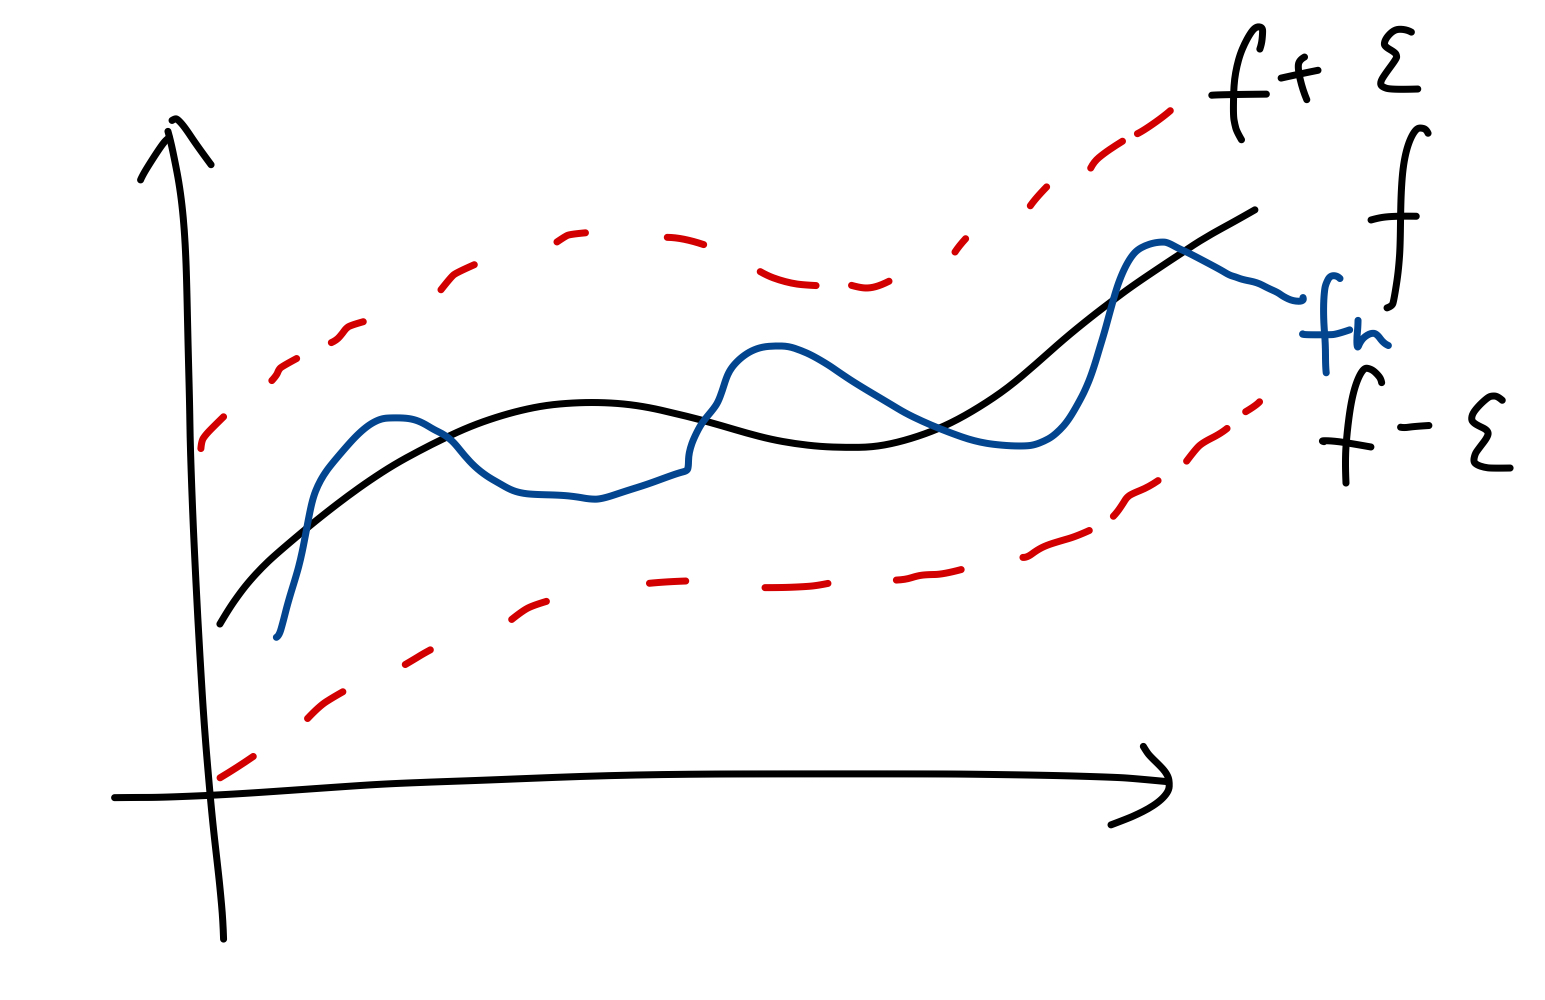
\includegraphics[scale=0.11]{at1.jpeg}
    \end{center}
\end{definition}

\begin{remark}\
    \begin{enumerate}
        \item $ N $ only depends on $\epsilon$!
        \item Uniform convergence implies pointwise convergence.
        \item Can replace $\mathbb{R}$ with $\mathbb{C}$ and can restrict to a subset of the domain.
        \item An equivalent definition of $f_{n} \rightarrow f$ uniformly on $S$ :
        \[
        \forall \varepsilon>0 \quad \exists N \in \mathbb{N} \quad \forall n \geqslant N \quad \sup _{x \in S}\left|f_{n}(x)-f(x)\right|<\varepsilon
        \]
        Even shorter: $\sup _{x \in S}\left|f_{n}(x)-f(x)\right| \rightarrow 0$ as $n \rightarrow \infty$
        \item The uniform limit $f$ if exists is unique.
    \end{enumerate}
\end{remark}

\begin{example}
\begin{enumerate}
    \item $f_{n}(x)=x^{2} \cdot e^{-n x}$ for $x \in[0, \infty)$, and $n \in \mathbb{N}$. We saw that $f_{n} \rightarrow f=0$ pointwise on $[0, \infty)$.
    \[
    0 \leqslant f_{n}(x)=\frac{x^{2}}{e^{n x}}=\frac{x^{2}}{1+n x+\frac{n^{2} x^{2}}{2}+\ldots} \leqslant \frac{2}{n^2}
    \]
    Thus,
    \[
    \sup _{x \in[0, \infty)}\left|f_{n}(x)-f(x)\right|=\sup _{x \in[0, \infty)} f_{n}(x) \leqslant \frac{2}{n^{2}} \rightarrow 0 \quad \text { as } \quad n \rightarrow \infty
    \]
    So $f_{n} \rightarrow 0$ uniformly on $[0, \infty)$.

    Could have used differentiation above to find the supremum, but the above method of finding an upper bound is better.
    \item $f_{n}(x)=x^{n}$ for $x \in[0,1], n \in \mathbb{N}$.
    We know that $f_{n} \rightarrow f$ pointwise on $[0,1]$, where
    \[
        f(x)= \begin{cases}0 & \text { if } 0 \leqslant x<1 \\ 1 & \text { if } x=1\end{cases}.
    \]
    Let $\varepsilon=1 / 2$. For any $n \in \mathbb{N}$, setting $x=\varepsilon^{1 / n}$, we have $f_{n}(x)=\varepsilon$, and so $\left|f_{n}(x)-f(x)\right| \geqslant \varepsilon$. So $f_{n} \not \rightarrow  f$ uniformly on $[0,1]$.

    Better: Since $f_{n}(1)=1$ and $f_{n}$ is continuous, there exist $\delta>0$ such that $\left|f_{n}(x)-1\right|<1 / 2$ for $x \in(1-\delta, 1+\delta)$. So for any $x \in[0,1]$ with $1-\delta<x<1$, we have $\left|f_{n}(x)-f(x)\right| \geqslant \varepsilon$.
\end{enumerate}
\end{example}
Q: Does $\left(f_{n}\right)$ converge uniformly on $S ?$
\subsection*{Strategy}
First check if $\left(f_{n}\right)$ converges pointwise on $S$.

If it doesn't, then $\left(f_{n}\right)$ does not converge uniformly on $S$.

If it does, then compute the pointwise limit $f$, and then it remains to check whether
\[
\sup _{x \in S}\left|f_{n}(x)-f(x)\right| \rightarrow 0 \quad \text { as } \quad n \rightarrow \infty
\]

If the above holds, then $f_{n} \rightarrow f$ uniformly on $S$, otherwise $\left(f_{n}\right)$ does not converge uniformly on $S$.

\begin{remark}
    What does it mean that $f_{n} \not \rightarrow f$ uniformly on $S$? We have to negate the sentence
    \[
    \forall \varepsilon>0 \quad \exists N \in \mathbb{N} \quad \forall n \geqslant N \quad \forall x \in S \quad\left|f_{n}(x)-f(x)\right|<\varepsilon
    \]
    The negation is
    \[
    \exists \varepsilon>0 \quad \forall N \in \mathbb{N} \quad \exists n \geqslant N \quad \exists x \in S \quad\left|f_{n}(x)-f(x)\right| \geqslant \varepsilon
    \]
\end{remark}

\subsection{Continuity, differentiability, and integrability}

The next theorem says that uniform limit of continuous functions is continuous.
\begin{theorem}\label{thm:1}
    Let $S$ be a subset of $\mathbb{R}$ or $\mathbb{C}$. Assume $f_{n} \rightarrow f$ uniformly on $S$. If $f_{n}$ is continuous for every $n \in \mathbb{N}$, then $f$ is continuous.
\end{theorem}
\textit{Idea}: Given $a \in S$, we want that $f(x) \approx f(a)$ provided $x \approx a$. We first choose large $n$ so that $f_{n}(x) \approx f(x)$ for every $x \in S$. Since $f_{n}$ is continuous, we have $f_{n}(x) \approx f_{n}(a)$ provided $x \approx a$. Thus, if $x \approx a$, then $f(x) \approx f_{n}(x) \approx f_{n}(a) \approx f(a)$.

\begin{proof}
    Fix $ a\in S, \epsilon>0 $. The goal is to find a $ \delta $ s.t. 
    \[
        \forall x\in S\quad |x-a|<\delta \Longrightarrow |f(x)-f(a)|<\epsilon.
    \]
    Since $ f_n\to f $ uniformly on $S$, $ \exists n\in \mathbb{N} $ such that 
    \[
        \forall x\in S\quad |f_n(x)-f(x)|<\epsilon.
    \]
    Since $f_n$ is continuous, $ \exists \delta>0 $, 
    \[
        \forall x\in S\quad |x-a|<\delta \Longrightarrow |f_n(x)-f_n(a)|<\epsilon.
    \]
    Thus for any $x\in S$, if $ |x-a|<\delta $,
    \[
        |f(x)-f(a)|\le |f(x)-f_n(x)|+|f_n(x)-f_n(a)|+|f_n(a)-f(a)|<3\epsilon.\qedhere
    \]
\end{proof}
\begin{remark}
    \begin{enumerate}
        \item It is not true for pointwise convergence. A counterexample is $x^n$.
        \item The result does not extend to differentiability.
        \item It follows that $x^{n}$ does not converge uniformly on $[0,1]$.
        \item The above proof is sometimes called a $3 \varepsilon$-proof.
        \item $\displaystyle \lim _{x \rightarrow a} \lim _{n \rightarrow \infty} f_{n}(x)=\lim _{x \rightarrow a} f(x)=f(a)=\lim _{n \rightarrow \infty} f_{n}(a)=\lim _{n \rightarrow \infty} \lim _{x \rightarrow a} f_{n}(x)$. i.e. we can \textit{swap limits} for uniformly convergent functions.
    \end{enumerate}
\end{remark}

\begin{lemma}\label{lemma 2}
    Let $S$ be any set and $f_{n}$ be a bounded function on $S$ for every $n \in \mathbb{N}$. If $f_{n} \rightarrow f$ uniformly on $S$, then $f$ is also bounded on $S$.
\end{lemma}
\begin{proof}
    Fix $n \in \mathbb{N}$ so that $\left|f_{n}(x)-f(x)\right| \leqslant 1$ for every $x \in S$. We can do this, since $f_{n} \rightarrow f$ uniformly on $S$. Since $f_{n}$ is bounded, there is an $M \in \mathbb{R}$ such that $\left|f_{n}(x)\right| \leqslant M$ for every $x \in S$. It follows that for every $x \in S$, we have
    \[
    |f(x)| \leqslant\left|f(x)-f_{n}(x)\right|+\left|f_{n}(x)\right| \leqslant 1+M
    \]
    Thus, $f$ is bounded by $M+1$.
\end{proof}

Before the next theorem, we recall some definitions and results from Analysis I. Assume $f:[a, b] \rightarrow \mathbb{R}$ is a bounded function. Given a dissection $\mathcal{D}: a=x_{0}<x_{1}<\cdots<x_{n}=b$ of $[a, b]$, the upper and lower sums of $f$ with respect to $\mathcal{D}$ are defined as
\[
U_{\mathcal{D}}(f)=\sum_{k=1}^{n}\left(x_{k}-x_{k-1}\right) \sup _{\left[x_{k-1}, x_{k}\right]} f \quad \text { and } \quad L_{\mathcal{D}}(f)=\sum_{k=1}^{n}\left(x_{k}-x_{k-1}\right) \inf _{\left[x_{k-1}, x_{k}\right]} f
\]
Riemann's criterion states that $f$ is integrable if and only if for every $\varepsilon>0$ there is a dissection $\mathcal{D}$ of $[a, b]$ such that
\[
U_{\mathcal{D}}(f)-L_{\mathcal{D}}(f)=\sum_{k=1}^{n}\left(x_{k}-x_{k-1}\right)\left(\sup _{\left[x_{k-1}, x_{k}\right]} f-\inf _{\left[x_{k-1}, x_{k}\right]} f\right)<\varepsilon
\]
An easy exercise shows that for an interval $I \subset[a, b]$ we have
\[
\sup _{I} f-\inf _{I} f=\sup _{x, y \in I}(f(x)-f(y))=\sup _{x, y \in I}|f(x)-f(y)|
\]
(This quantity is sometimes called the oscillation of $f$ on $I$.)

\begin{theorem}\label{theorem 3}
    Assume $f_{n}:[a, b] \rightarrow \mathbb{R}$ is Riemann-integrable for every $n \in \mathbb{N}$. If $f_{n} \rightarrow f$ uniformly on $[a, b]$, then $f$ is also Riemann-integrable on $[a, b]$, and moreover
    \[
    \int_{a}^{b} f_{n} \rightarrow \int_{a}^{b} f \quad \text { as } n \rightarrow \infty.
    \]
\end{theorem}

\begin{proof}
    We are going to prove that $f$ is bounded and that it satisfies Riemann's criterion. By definition of integrability, each $f_{n}$ is bounded, and hence so is $f$ by Lemma \ref{lemma 2}.
    Next, fix $\varepsilon>0$. Since $f_{n} \rightarrow f$ uniformly on $[a, b]$, we can fix $n \in \mathbb{N}$ so that $\left|f_{n}(x)-f(x)\right|<\varepsilon$ for all $x \in[a, b]$. Since $f_{n}$ is integrable, it satisfies Riemann's criterion, so there is a dissection $\mathcal{D}$ of $[a, b]$ such that $U_{\mathcal{D}}\left(f_{n}\right)-L_{\mathcal{D}}\left(f_{n}\right)<\varepsilon$. If $I$ is one of the sub-intervals of $\mathcal{D}$, then for any $x, y \in I$ we have
    \[
    \begin{aligned}
    |f(x)-f(y)| & \leqslant\left|f(x)-f_{n}(x)\right|+\left|f_{n}(x)-f_{n}(y)\right|+\left|f_{n}(y)-f(y)\right| \\
    &<\left|f_{n}(x)-f_{n}(y)\right|+2 \varepsilon
    \end{aligned}
    \]
    It follows that
    \[
    \sup _{x, y \in I}|f(x)-f(y)| \leqslant \sup _{x, y \in I}\left|f_{n}(x)-f_{n}(y)\right|+2 \varepsilon
    \]
    Multiplying both sides with the length of $I$ and summing over all sub-intervals $I$ of $\mathcal{D}$, we obtain
    \[
    U_{\mathcal{D}}(f)-L_{\mathcal{D}}(f) \leqslant U_{\mathcal{D}}\left(f_{n}\right)-L_{\mathcal{D}}\left(f_{n}\right)+2 \varepsilon(b-a)<(2(b-a)+1) \varepsilon.
    \]
    So $f$ satisfies Riemann's criterion, and thus, $f$ is integrable.
    Finally, we estimate
    \[
    \left|\int_{a}^{b} f_{n}-\int_{a}^{b} f\right| \leqslant \int_{a}^{b}\left|f_{n}-f\right| \leqslant(b-a) \sup _{[a, b]}\left|f_{n}-f\right| \rightarrow 0 \quad \text { as } n \rightarrow \infty .\qedhere
    \]
\end{proof}
\begin{remark}
    $\int_{a}^{b} \lim _{n \rightarrow \infty} f_{n}(x) \mathrm{d} x=\lim _{n \rightarrow \infty} \int_{a}^{b} f_{n}(x) \mathrm{d} x$. i.e. for uniformly convergent functions we can swap limits and integrals.
\end{remark}

\begin{corollary}\label{col:4}
    Let $f_{n}:[a, b] \rightarrow \mathbb{R}$ be an integrable function for each $n \in \mathbb{N}$. If $\sum_{n=1}^{\infty} f_{n}(x)$ converges uniformly on $[a, b]$, then $\sum_{n=1}^{\infty} f_{n}(x)$ defines an integrable function on $[a, b]$, and moreover
    \[
    \int_{a}^{b} \sum_{n=1}^{\infty} f_{n}(x) \mathrm{d} x=\sum_{n=1}^{\infty} \int_{a}^{b} f_{n}(x) \mathrm{d} x.
    \]
\end{corollary}
\begin{proof}
    Define $F_{n}(x)=\sum_{k=1}^{n} f_{k}(x)$ for $x \in[a, b]$ and $n \in \mathbb{N}$. To say that $\sum_{n=1}^{\infty} f_{n}(x)$ converges uniformly on $[a, b]$ means that $\left(F_{n}\right)$ converges uniformly on $[a, b]$. So for each $x \in[a, b]$, the series $\sum_{n=1}^{\infty} f_{n}(x)$ is convergent, and the function $x \mapsto \sum_{n=1}^{\infty} f_{n}(x)$ is the uniform limit of $\left(F_{n}\right)$ on $[a, b]$.

    We know that each $F_{n}$ is integrable and $\int_{a}^{b} F_{n}=\sum_{k=1}^{n} \int_{a}^{b} f_{k}$. So by Theorem 3 , the function $\sum_{n=1}^{\infty} f_{n}(x)$ is integrable and
    \[
    \int_{a}^{b} \sum_{n=1}^{\infty} f_{n}(x) \mathrm{d} x=\lim _{n \rightarrow \infty} \int_{a}^{b} F_{n}(x) \mathrm{d} x=\lim _{n \rightarrow \infty} \sum_{k=1}^{n} \int_{a}^{b} f_{k}(x) \mathrm{d} x=\sum_{k=1}^{\infty} \int_{a}^{b} f_{k}(x) \mathrm{d} x.\qedhere
    \]
\end{proof}

However, even uniform convergence does not guarantee differentiability. 
\begin{example}
    Let 
    \[
        f_n(x) = \begin{cases}
        |x| &\text{if }|x|\ge \frac{1}{n}\\
        \frac{n}{2}x^2+\frac{1}{2n} &\text{if }|x|<\frac{1}{n}\\
        \end{cases} \quad f(x) = |x|
    \]
    Then $ f_n\to f $ uniformly, but $f$ is not differentiable at $0$. 

    Indeed, if $ |x|\ge \frac{1}{n}, |f_n(x)-f(x)|=0 $. If $ |x|<\frac{1}{n} $, we have 
    \begin{align*}
        |f_n(x)-f(x)| &= \left| \frac{n}{2}x^2+\frac{1}{2n}-|x| \right| \\ 
        &\le \frac{n}{2}x^2+\frac{1}{2n} +|x| \\ 
        &\le \frac{n}{2}\left( \frac{1}{n} \right) +\frac{1}{2n}+\frac{1}{n}
        =\frac{2}{n}. 
    \end{align*}
    So 
    \[
        \sup_{x\in (-1,1)}|f_n(x)-f(x)| \le \frac{2}{n}\to 0, 
    \]
    and $f_n\to f$ uniformly. 
\end{example}

\begin{theorem}\label{thm:5}
    Let $\left(f_{n}\right)$ be a sequence of continuously differentiable functions on $[a, b]$. Assume further that
    \begin{enumerate}
        \item $\sum_{n=1}^{\infty} f_{n}^{\prime}(x)$ converges uniformly on $[a, b]$;
        \item there exists $c \in[a, b]$ such that $\sum_{n=1}^{\infty} f_{n}(c)$ converges.
    \end{enumerate}
    Then $\sum_{n=1}^{\infty} f_{n}(x)$ converges uniformly to a continuously differentiable function $f$ on $[a, b]$, and moreover, we have
    \[
    f^{\prime}(x)=\sum_{n=1}^{\infty} f_{n}^{\prime}(x) \quad \text { for all } x \in[a, b].
    \]
\end{theorem}
\begin{note}
    Informally, $\displaystyle \frac{\mathrm{d}}{\mathrm{d}x}\left( \sum_{n=1}^{\infty}f_n(x) \right) = \sum_{n=1}^{\infty}\frac{\mathrm{d}f_n}{\mathrm{d}x}  $. 
\end{note}
\begin{proof}
    Let $g(x)=\sum_{n=1}^{\infty} f_{n}^{\prime}(x)$ for $x \in[a, b]$. Idea: solve the equation $f^{\prime}=g$ with initial condition $f(c)=\sum_{n=1}^{\infty} f_{n}(c)$.

    Since $\sum_{n=1}^{\infty} f_{n}^{\prime}(x)$ converges uniformly to $g(x)$, and since $f_{n}^{\prime}$ is continuous for every $n \in \mathbb{N}$, by Theorem \ref{thm:1}, $ g$ is continuous, and hence integrable. Let $\lambda=\sum_{n=1}^{\infty} f_{n}(c)$ and define
    \[
    f(x)=\lambda+\int_{c}^{x} g(t)\, \mathrm{d} t \quad \text { for } x \in[a, b]
    \]
    Since $g$ is continuous, by the Fundament Theorem of Calculus (FTC) $f$ is differentiable with $f^{\prime}=g$, and moreover $f(c)=\lambda$. By the FTC we also have
    \[
    f_{k}(x)=f_{k}(c)+\int_{c}^{x} f_{k}^{\prime}(t)\, \mathrm{d} t \quad \text { for } x \in[a, b], k \in \mathbb{N}
    \]
    Given $\varepsilon>0$, by our assumptions there exists $N \in \mathbb{N}$ such that
    \[
    \begin{array}{rll}
    \displaystyle \left|\lambda-\sum_{k=1}^{n} f_{k}(c)\right| & <\varepsilon & \forall n \geqslant N \\[15pt]
    \displaystyle \left|g(t)-\sum_{k=1}^{n} f_{k}^{\prime}(t)\right| & <\varepsilon & \forall n \geqslant N \quad \forall t \in[a, b]
    \end{array}
    \]
    It follows that for all $n \geqslant N$ and for all $x \in[a, b]$ we have
    \[
    \begin{aligned}
    \left|f(x)-\sum_{k=1}^{n} f_{k}(x)\right| &=\left|\lambda+\int_{c}^{x} g(t)\, \mathrm{d} t-\sum_{k=1}^{n}\left(f_{k}(c)+\int_{c}^{x} f_{k}^{\prime}(t) \,\mathrm{d} t\right)\right| \\
    &=\left|\lambda-\sum_{k=1}^{n} f_{k}(c)+\int_{c}^{x}\left(g(t)-\sum_{k=1}^{n} f_{k}^{\prime}(t)\right) \mathrm{d} t\right| \\
    & \leqslant\left|\lambda-\sum_{k=1}^{n} f_{k}(c)\right|+\left|\int_{c}^{x}\left(g(t)-\sum_{k=1}^{n} f_{k}^{\prime}(t)\right) \mathrm{d} t\right| \\
    &<\varepsilon+(b-a) \varepsilon.
    \end{aligned}
    \]
    This shows that $\sum_{k=1}^{n} f_{k}(x) \rightarrow f(x)$ uniformly on $[a, b]$. We have already seen that $f$ is differentiable and $f^{\prime}=g$ is continuous.
\end{proof}

By considering partial sums in theorem \ref{thm:5} we get 
\begin{theorem}
    Let $(f_n)$ be a sequence of continuously differentiable functions on $[a,b]$ and assume that 
    \begin{enumerate}
        \item $f'_n$ converges uniformly to $g$ on $[a,b]$, 
        \item $f_n$ converges pointwise to $f$.
    \end{enumerate}
    Then $f$ is differentiable and $ f'=g $. 
\end{theorem}

\subsection{Uniform Cauchy}

We recall from Analysis I: a scalar sequence $\left(x_{n}\right)$ is Cauchy if
\[
\forall \varepsilon>0 \quad \exists N \in \mathbb{N} \quad \forall m, n \geqslant N \quad\left|x_{m}-x_{n}\right|<\varepsilon.
\]
The General Principle of Convergence (GPC): every Cauchy sequence is convergent.
\begin{definition}
    Let $\left(f_{n}\right)$ be a sequence of scalar functions on a set $S$. We say $\left(f_{n}\right)$ is uniformly Cauchy on $S$ if
    \[
    \forall \varepsilon>0 \quad \exists N \in \mathbb{N} \quad \forall m, n \geqslant N \quad \forall x \in S \quad\left|f_{m}(x)-f_{n}(x)\right|<\varepsilon.
    \]
\end{definition}

\begin{theorem}[General Principle of Uniform Convergence (GPUC)]\label{thm:6}
    If $\left(f_{n}\right)$ is a uniformly Cauchy sequence of scalar functions on a set $S$, then $\left(f_{n}\right)$ converges uniformly to some function $f$ on $S$.
\end{theorem}

\begin{proof}
    We first show that $\left(f_{n}\right)$ converges pointwise on $S$. Fix $x \in S$. Given $\varepsilon>0$ since $\left(f_{n}\right)$ is uniformly Cauchy, there exists $N \in \mathbb{N}$ such that
    \[
    \forall m, n \geqslant N \quad \forall t \in S \quad\left|f_{m}(t)-f_{n}(t)\right|<\varepsilon.
    \]
    In particular, for all $m, n \geqslant N$, we have $\left|f_{m}(x)-f_{n}(x)\right|<\varepsilon$. Thus, $\left(f_{n}(x)\right)_{n=1}^{\infty}$ is a Cauchy sequence, and hence convergent by the GPC. Set $f(x)=\lim _{n \rightarrow \infty} f_{n}(x)$. Doing this for every $x \in S$, we obtain a function $f$ on $S$.
    We claim that $f_{n} \rightarrow f$ uniformly on $S$. Then we will be done. 
    
    Given $\varepsilon>0$, since $\left(f_{n}\right)$ is uniformly Cauchy, there exists $N \in \mathbb{N}$ such that
    \[
    \forall m, n \geqslant N \quad \forall x \in S \quad\left|f_{m}(x)-f_{n}(x)\right|<\varepsilon.
    \]
    Fix $n \geqslant N$ and $x \in S$. Since $\left|f_{m}(x)-f_{n}(x)\right|<\varepsilon$ for every $m \geqslant N$, letting $m \rightarrow \infty$, we obtain $\left|f(x)-f_{n}(x)\right| \leqslant \varepsilon$. Since this holds for every $n \geqslant N$ and for every $x \in S$, we are done.
\end{proof}
\begin{theorem}[The Weierstrass $M$-test]\label{thm:7}
    Let $\left(f_{n}\right)$ be a sequence of scalar functions on a set $S$. Let $\sum_{n} M_{n}$ be a convergent series of non-negative real numbers. Assume that $\left|f_{n}(x)\right| \leqslant M_{n}$ for every $x \in S$ and $n \in \mathbb{N}$. Then $\sum_{n} f_{n}(x)$ converges uniformly on $S$.
\end{theorem}
\begin{proof}
    Set $F_{n}(x)=\sum_{k=1}^{n} f_{k}(x)$ for $x \in S$ and $n \in \mathbb{N}$. For $n \geqslant m$ and $x \in S$ we have
    \[
    \left|F_{m}(x)-F_{n}(x)\right| \leqslant\left|\sum_{k=m+1}^{n} f_{k}(x)\right| \leqslant \sum_{k=m+1}^{n}\left|f_{k}(x)\right| \leqslant \sum_{k=m+1}^{n} M_{k}
    \]
    Given $\varepsilon>0$, choose $N \in \mathbb{N}$ such that $\sum_{k=N}^{\infty} M_{k}<\varepsilon$. Then by the above, for every $x \in S$ and every $n \geqslant m \geqslant N$ in $\mathbb{N}$, we have
    \[
    \left|F_{m}(x)-F_{n}(x)\right| \leqslant \sum_{k=m+1}^{n} M_{k}<\varepsilon
    \]
    So $\left(F_{n}\right)$ is uniformly Cauchy, and hence uniformly convergent by Theorem \ref{thm:6}.
\end{proof}

\begin{definition}
    Let $X \subseteq \mathbb{R}$ and let $f_n:X\to \mathbb{R}$ for each $n\ge 1$. We say $(f_n)$ is \textbf{pointwise bounded} if 
    \[
        \exists M\quad \forall n\quad |f_n(x)|\le M. 
    \]
    We say $(f_n)$ is \textbf{uniformly bounded} if 
    \[
        \exists M \quad \forall x\quad \forall n \quad |f_n(x)|\le M. 
    \]
\end{definition}

\begin{note}
    Bolzano-Weierstrass theorem DOES NOT work (in uniform context). A counterexample is 
    \[
        f_n(x) = \begin{cases}
        1 &\text{if }x = n\\
        0 &\text{if }x\neq n\\
        \end{cases} 
    \]
\end{note}

\subsection{Application in power series}

Consider a power series $\sum_{n=0}^{\infty} c_{n}(z-a)^{n}$. Here $\left(c_{n}\right)_{n=0}^{\infty}$ is a complex sequence, a, $z \in \mathbb{C}$. We think of $\left(c_{n}\right)$ and $a$ as fixed, and $z$ as a variable.
Let $R$ be the radius of convergence of this power series. This means:
$|z-a|<R \quad \Longrightarrow \quad \sum_{n=0}^{\infty} c_{n}(z-a)^{n}$ converges absolutely, and hence converges, $|z-a|>R \Longrightarrow \sum_{n=0}^{\infty} c_{n}(z-a)^{n}$ diverges.

Denote $D(a, R)=\{z \in \mathbb{C}:|z-a|<R\}$, the open disk of centre $a$ and radius $R$. Consider the function
\[
f: D(a, R)  \rightarrow \mathbb{C},\quad
f(z) =\sum_{n=0}^{\infty} c_{n}(z-a)^{n}.
\]
The power series converges pointwise to $f$.

Q: Does the power series converge uniformly inside the radius of convergence?

A: In general, NO.

\begin{example}
\begin{enumerate}
    \item $\sum_{n=1}^{\infty} \frac{z^{n}}{n^{2}}$ for $|z|<1$
    Consider $f_{n}: D(0,1) \rightarrow \mathbb{C}$ define by $f_{n}(z)=z^{n} / n^{2}$. Note that $\left|f_{n}(z)\right| \leqslant 1 / n^{2}$ for all $|z|<1$. Moreover, $\sum_{n=1}^{\infty} \frac{1}{n^{2}}$ converges. Hence by the Weierstrass $M$-test, the power series converges uniformly on $D(0,1)$.
    
    \item $\sum_{n=0}^{\infty} z^{n}=\frac{1}{1-z}$ for $|z|<1$.
    $\left|\sum_{n=0}^{N} z^{n}\right| \leqslant N+1$ for $|z|<1$ and $N \in \mathbb{N} .$ So the partial sum functions are bounded on $D(0,1)$. However, $\frac{1}{1-z}$ is not bounded on $D(0,1)$. By Lemma \ref{lemma 2}, the convergence cannot be uniform on $D(0,1)$.
    Alternatively,
    \[
    \sup _{|z|<1}\left|\sum_{n=0}^{N} z^{n}-\frac{1}{1-z}\right|=\sup _{|z|<1}\left|\frac{z^{N+1}}{1-z}\right|=\infty.
    \]
\end{enumerate}
\end{example}
\begin{theorem}\label{thm:8}
    Let $\sum_{n=0}^{\infty} c_{n}(z-a)^{n}$ be a power series with radius of convergence $R$. Then for any $r$ with $0<r<R$, the power series $\sum_{n=0}^{\infty} c_{n}(z-a)^{n}$ converges uniformly on $D(a, r)=\{z \in \mathbb{C}:|z-a|<r\}$
\end{theorem}
\begin{proof}
    Fix $w \in D(a, R)$ with $r<|w-a|<R$. (E.g., $\left.w=a+\frac{r+R}{2} .\right)$ Set $\rho=\frac{r}{|w-a|}$. Since $\sum_{n=0}^{\infty} c_{n}(w-a)^{n}$ converges, we must have $c_{n}(w-a)^{n} \rightarrow 0$ as $n \rightarrow \infty$. It follows that the sequence $\left(c_{n}(w-a)^{n}\right)_{n=0}^{\infty}$ is bounded. Thus, there exists $M \geqslant 0$ such that $\left|c_{n}(w-a)^{n}\right| \leqslant M$ for all $n \geqslant 0$. Now, for any $z \in D(a, r)$ and $n \in \mathbb{N}$, we have
    \[
    \left|c_{n}(z-a)^{n}\right|=\left|c_{n}(w-a)^{n}\right| \cdot\left|\frac{(z-a)^{n}}{(w-a)^{n}}\right| \leqslant M \frac{r^{n}}{|(w-a)|^{n}}=M \rho^{n}
    \]
    Since $\sum_{n=0}^{\infty} M \rho^{n}$ converges, by Theorem \ref{thm:7}(the Weierstrass $M$-test) the power series $\sum_{n=0}^{\infty} c_{n}(z-a)^{n}$ converges uniformly on $D(a, r)=\{z \in \mathbb{C}:|z-a|<r\}$.
\end{proof}
\begin{remark}
    \begin{enumerate}
        \item The function $f: D(a, R) \rightarrow \mathbb{C}, f(z)=\sum_{n=0}^{\infty} c_{n}(z-a)^{n}$ is continuous on $D(a, r)$ for any $0<r<R$ being the uniform limit of continuous functions (polynomials). This is by Theorem \ref{thm:1}. Since $D(a, R)=\bigcup_{0<r<R} D(a, r), f$ is continuous on $D(a, R)$.
        
        \item  The power series $\sum_{n=1}^{\infty} c_{n} n(z-a)^{n-1}$ also has radius of convergence $R$ (from Analysis I). Hence it converges uniformly on $D(a, r)$ for any $0<r<R$. By an analogue of Theorem \ref{thm:5} we can deduce that $f$ is complex differentiable on $D(a, R)$ and
        \[
        f^{\prime}(z)=\frac{\mathrm{d}}{\mathrm{d} z}\left(\sum_{n=0}^{\infty} c_{n}(z-a)^{n}\right)=\sum_{n=1}^{\infty} c_{n} n(z-a)^{n-1}
        \]
        See Complex Analysis.
    
        \item Given $w \in D(a, R)$, fix $r$ with $|w-a|<r<R$ and $\delta>0$ with $|w-a|+\delta<r$. Then $D(w, \delta) \subset D(a, r) .$ Indeed, given $z \in D(w, \delta)$,
        \[
        |z-a| \leqslant|z-w|+|w-a|<\delta+|w-a|<r
        \]
        So $z \in D(a, r)$. It follows that the power series $\sum_{n=0}^{\infty} c_{n}(z-a)^{n}$ converges uniformly on $D(w, \delta)$.
    \end{enumerate}
\end{remark}
\begin{definition}
    A subset $U$ of $\mathbb{C}$ is open if for every $w \in U$ there is a $\delta>0$ such that $D(w, \delta) \subset U$
\end{definition}

\begin{definition}
    Let $U$ be an open subset of $\mathbb{C}$. A sequence $\left(f_{n}\right)$ of scalar functions on $U$ converges \textit{locally uniformly} on $U$ if for every $w \in U$ there is a $\delta>0$ such that $D(w, \delta) \subset U$ and $f_{n} \rightarrow f$ uniformly on $D(w, \delta)$
\end{definition}

\begin{remark}
    \begin{enumerate}
        \item We will return to this concept after covering compactness.
        \item Above we proved that a power series converges locally uniformly inside the radius of convergence.
    \end{enumerate}
\end{remark}

\subsection{Uniform Continuity}
We next turn to the topic of Uniform Continuity. We begin by recalling the notion of continuity from Analysis I.
Let $U$ be a subset of $\mathbb{R}$ or $\mathbb{C}$ and let $f$ be a scalar function on $U$. For $x \in U$, we say $f$ is continuous at $x$ if
\[
\forall \varepsilon>0 \quad \exists \delta>0 \quad \forall y \in U \quad|y-x|<\delta \Longrightarrow|f(y)-f(x)|<\varepsilon.
\]
We say $f$ is continuous on $U$ if $f$ is continuous at $x$ for every $x \in U$, i.e.,
\[
    \forall x \in U \quad \forall \varepsilon>0 \quad \exists \delta>0 \quad \forall y \in U \quad|y-x|<\delta \Longrightarrow|f(y)-f(x)|<\varepsilon.
\]
\begin{note}
    $\delta$ depends on $\varepsilon$ and on $x$.
\end{note}

\begin{definition}
    Let $U$ be a subset of $\mathbb{R}$ or $\mathbb{C}$ and let $f$ be a scalar function on $U$. We say $f$ is uniformly continuous on $U$ if
\[
\forall \varepsilon>0 \quad \exists \delta>0 \quad \forall x, y \in U \quad|y-x|<\delta \Longrightarrow|f(y)-f(x)|<\varepsilon
\]
\end{definition}

\begin{note}
    $\delta$ depends only on $\varepsilon$. So uniform continuity implies continuity.
\end{note}

\begin{example}
    \begin{enumerate}
        \item Consider $f: \mathbb{R} \rightarrow \mathbb{R}, f(x)=2x+17$. Given $\varepsilon>0$, set $\delta=\varepsilon / 2$. Then for every $x, y \in \mathbb{R}$, if $|x-y|<\delta$, then
        \[
        |f(x)-f(y)|=2|x-y|<2 \delta=\varepsilon
        \]
        So $f$ is uniformly continuous on $\mathbb{R}$.
        \item Consider $f: \mathbb{R} \rightarrow \mathbb{R}, f(x)=x^{2}$. Given $\varepsilon=1$, we try to find $\delta>0$ that works. Consider any $x>0$ and $y=x+\frac{\delta}{2}$. Then $|x-y|=\delta / 2<\delta$ and
        \[
        |f(x)-f(y)|=(x+\delta / 2)^{2}-x^{2}=x \delta+\delta^{2} / 4
        \]
        So for any $\delta>0$, if $x=1 / \delta$ and $y=x+\delta / 2$, then $|x-y|<\delta$ but $|f(x)-f(y)|>\varepsilon$. So $f$ is not uniformly continuous, but $f$ is continuous on $\mathbb{R}$.
    \end{enumerate}
\end{example}

\begin{note}
    A function $f$ on a subset $U$ of $\mathbb{R}$ or $\mathbb{C}$ is NOT uniformly continuous if
    \[
        \forall \varepsilon>0 \quad \exists \delta>0 \quad \forall x, y \in U \quad|x-y|<\delta \Longrightarrow|f(x)-f(y)|<\varepsilon
    \]
    is FALSE, that is
    \[
        \exists \varepsilon>0 \quad \forall \delta>0 \quad \exists x, y \in U \quad|x-y|<\delta \text{ and }|f(x)-f(y)| \geqslant \varepsilon
    \]
\end{note}
\begin{theorem}\label{thm:9}
    Let $f$ be a scalar function on a closed, bounded interval $[a, b]$. If $f$ is continuous on $[a, b]$, then $f$ is uniformly continuous on $[a, b]$. 
\end{theorem}
One idea: Let $\varepsilon>0$. For each $x \in[a, b]$ there is a $\delta_{x}>0$ such that if $|y-x|<\delta_{x}$ then $|f(y)-f(x)|<\varepsilon$. We want to take $\delta=\inf _{x} \delta_{x} .$ We might have $\delta=0$. Instead, we work indirectly: argue by contradiction.
\begin{proof}
    Assume there is an $\varepsilon>0$ such that
    \[
        \forall \delta>0 \quad \exists x, y \in[a, b] \quad|x-y|<\delta \text{ and }|f(x)-f(y)| \geqslant \varepsilon
    \]
    In particular, for every $n \in \mathbb{N}$, there exist $x_{n}, y_{n} \in[a, b]$ such that $\left|x_{n}-y_{n}\right|<1 / n$ and $\left|f\left(x_{n}\right)-f\left(y_{n}\right)\right| \geqslant \varepsilon$. By Bolzano-Weierstrass there is a subsequence $\left(x_{k_{n}}\right)_{n}$ of $\left(x_{n}\right)$ that converges to some $x \in[a, b]$. Then
    \[
    \left|y_{k_{n}}-x\right| \leqslant\left|y_{k_{n}}-x_{k_{n}}\right|+\left|x_{k_{n}}-x\right| \leqslant 1 / n+\left|x_{k_{n}}-x\right| \rightarrow 0
    \]
    Since $f$ is continuous at $x, f\left(x_{k_{n}}\right) \rightarrow f(x)$ and $f\left(y_{k_{n}}\right) \rightarrow f(x)$. Hence 
    \[
        \varepsilon \leqslant\left|f\left(x_{k_{n}}\right)-f\left(y_{k_{n}}\right)\right| \rightarrow|f(x)-f(x)|=0,
    \]
    which is a contradiction.
\end{proof}
\begin{corollary}\label{col:10}
    Let $f:[a, b] \rightarrow \mathbb{R}$ be a continuous function. Then $f$ is integrable.
\end{corollary}
\begin{proof}
    $f$ is bounded since it is continuous on the closed bounded interval $[a, b]$. It remains to verify Riemann's criterion.

    Given $\varepsilon>0$, since $f$ is uniformly continuous by Theorem \ref{thm:9}, there is a $\delta>0$ such that $|f(x)-f(y)|<\varepsilon$ whenever $|x-y|<\delta$.
    
    Next, choose a dissection $\mathcal{D}$ of $[a, b]$ such that every subinterval of $\mathcal{D}$ has length strictly less than $\delta$. (E.g. choose $n$ with $\frac{b-a}{n}<\delta$ and let $\mathcal{D}$ consist of $a+k \frac{b-a}{n}, k=0,1, \ldots, n$.) If $I$ is a subinterval of $\mathcal{D}$, then for all $x, y \in I$, we have $|x-y|<\delta$, and hence $|f(x)-f(y)|<\varepsilon$. It follows that
    \[
    \sup _{1} f-\inf _{1} f=\underset{x, y \in I}{\sup }|f(x)-f(y)| \leqslant \varepsilon
    \]
    Multiplying both sides by the length of $I$, and summing over all $I$, we obtain
    \[
    U_{\mathcal{D}}(f)-L_{\mathcal{D}}(f) \leqslant(b-a) \varepsilon.\qedhere
    \]
\end{proof}

\section{Metric Spaces}
\subsection{Definition of metric spaces}
In $\mathbb{R}$ or $\mathbb{C}$, we measure the ``closeness'' of points $x$ and $y$ by the expression $|x-y|$. A frequently used property of this ``distance'' is the triangle-inequality. We will now generalize this concept.

\begin{definition}
    Let $M$ be a set. A \textit{metric} on $M$ is a function $d: M \times M \rightarrow \mathbb{R}$ satisfying
    \begin{enumerate}[(i)]
        \item $\forall x, y \in M, d(x, y) \geqslant 0$ and $d(x, y)=0 \Longleftrightarrow x=y$\hfill (positivity)
        \item $\forall x, y \in M, d(x, y)=d(y, x)$\hfill (symmetry)
        \item $\forall x, y, z \in M, d(x, z) \leqslant d(x, y)+d(y, z)$\hfill(triangle-inequality)
    \end{enumerate}
    A \textit{metric space} is a pair $(M, d)$, where $M$ is a set and $d$ is a metric on $M$.
\end{definition}
\begin{example}
    \begin{enumerate}
        \item $M=\mathbb{R}$ or $\mathbb{C},\ d(x, y)=|x-y|$. We refer to this as the usual metric on $M$ and will always be used unless otherwise stated.
        \item $M=\mathbb{R}^{n}$ or $\mathbb{C}^{n} .$ We define the euclidean norm or euclidean length of a vector $x \in M$ by
        \[
        \|x\|=\|x\|_{2}=\left(\sum_{k=1}^{n}\left|x_{k}\right|^{2}\right)^{1 / 2}
        \]
        This satisfies the inequality $\|x+y\| \leqslant\|x\|+\|y\|$. It follows that
        \[
        d(x, y)=d_{2}(x, y)=\|x-y\|=\left(\sum_{k=1}^{n}\left|x_{k}-y_{k}\right|^{2}\right)^{1 / 2}
        \]
        defines a metric on $M$ called the euclidean metric. E.g. we check the triangle-inequality:
        \[
        d(a, c)=\|a-c\|=\|a-b+b-c\| \leqslant\|a-b\|+\|b-c\|=d(a, b)+d(b, c).
        \]
        The resulting metric space $(M, d)$ is called $n$-dimensional real or complex Euclidean space. $M$ will always be equipped with the Euclidean metric unless otherwise stated. The metric space $(M, d)$ is sometimes denoted by $\ell_{2}^{n}$ and $d_{2}$ is also called the $\ell_{2}$-metric, and $\|\cdot\|_{2}$ is also called $\ell_{2}$-norm.
        \item $M=\mathbb{R}^{n}$ or $\mathbb{C}^{n} .$ We define the $\ell_{1}$-norm of a vector $x \in M$ by
        \[
        \|x\|_{1}=\sum_{k=1}^{n}\left|x_{k}\right|
        \]
        and the corresponding metric, called the $\ell_{1}$-metric, is given by
        \[
        d_{1}(x, y)=\|x-y\|_{1}=\sum_{k=1}^{n}\left|x_{k}-y_{k}\right|
        \]
        The metric space $\left(M, d_{1}\right)$ is denoted by $\ell_{1}^{n}$. It is not hard to see how to generalize this further. For any $1 \leqslant p<\infty$ one can define the $\ell_{p}$-norm by
        \[
        \|x\|_{p}=\left(\sum_{k=1}^{n}\left|x_{k}\right|^{p}\right)^{1 / p}
        \]
        and the corresponding $\ell_{p}$-metric by $d_{p}(x, y)=\|x-y\|_{p} .$ In this course, we will only deal with $p=1,2$. (For the general case, see Part II Linear Analysis).

        Question: How about $p=\infty ?$
        \item Letting $p \rightarrow \infty$ in the previous example leads to the $\ell_{\infty}$-norm and to the $\ell_{\infty}$-metric on $M=\mathbb{R}^{n}$ or $\mathbb{C}^{n}:$
        \[
        \|x\|_{\infty}=\max _{1 \leqslant k \leqslant n}\left|x_{k}\right|\quad \text {and}\quad d_{\infty}(x, y)=\|x-y\|_{\infty}=\max _{1 \leqslant k \leqslant n}\left|x_{k}-y_{k}\right|
        \]
        The metric space $\left(M, d_{\infty}\right)$ is denoted by $\ell_{\infty}^{n}$.
        \item Let $S$ be a set. We denote by $\ell_{\infty}(S)$ the set of all bounded scalar functions on $S$. We define the $\ell_{\infty}$-norm (or uniform norm, or sup norm) of a function $f \in \ell_{\infty}(S)$ by
        \[
        \|f\|=\|f\|_{\infty}=\sup \{|f(x)|: x \in S\}
        \]
        (The sup exists since $f$ is bounded: $\exists C \geqslant 0, \forall x \in S,|f(x)| \leqslant C$.) Note that for $f, g \in \ell_{\infty}(S)$ and for any $x \in S$, we have
        \[
        |f(x)+g(x)| \leqslant|f(x)|+|g(x)| \leqslant\|f\|+\|g\|
        \]
        and hence $\|f+g\| \leqslant\|f\|+\|g\|$. It follows that $d(f, g)=\|f-g\|_{\infty}$ defines a metric, called the uniform metric (or $\ell_{\infty}$-metric) on $\ell_{\infty}(S)$.
        
        Note that $\ell_{\infty}^{n}=\ell_{\infty}(\{1,2, \ldots, n\})$. Also, $\ell_{\infty}(\mathbb{N})$ is often denoted simply $\ell_{\infty}$. This is the space of bounded scalar sequences.
        \item $C[a, b]$ denotes the space of continuous scalar functions on the closed bounded interval $[a, b]$. Let $p=1$ or 2 . We define the $L_{p}$-norm on $C[a, b]$ by
        \[
        \|f\|_{p}=\left(\int_{a}^{b}|f(t)|^{p} \mathrm{~d} t\right)^{1 / p} \quad(f \in C[a, b])
        \]
        The corresponding metric $d_{p}(f, g)=\|f-g\|_{p}$ is the $L_{p}$-metric on $C[a, b]$. E.g., for $f, g \in C[a, b]$ we have
        \[
        \|f+g\|_{1}=\int_{a}^{b}|f+g| \leqslant \int_{a}^{b}|f|+|g|=\int_{a}^{b}|f|+\int_{a}^{b}|g|=\|f\|_{1}+\|g\|_{1}
        \]
        which implies the triangle-inequality for $d_{1}$.
        \item Let $M$ be any set. For $x, y \in M$ we define
        \[
        d(x, y)= \begin{cases}0 & \text { if } x=y \\ 1 & \text { if } x \neq y\end{cases}
        \]
        This is called the discrete metric on $M$ and $(M, d)$ is a discrete metric space.
        \item Let $G$ be a group generated by $S \subset G$. Then
        \[
        d(x, y)=\min \left\{n: \exists s_{1}, \ldots, s_{n} \in S,\ y=x s_{1} s_{2} \cdots s_{n}\right\}
        \]
        is a metric called the \textit{word metric} on $G$ (Geometric Group Theory).
        \item Fix a prime $p$ in $\mathbb{Z}$. For $x, y \in \mathbb{Z}$ write $x-y=p^{n} m$ where $m, n \in \mathbb{Z}, n \geqslant 0$ and $p \nmid m$; then define
        \[
        d(x, y)= \begin{cases}0 & \text { if } x=y \\ p^{-n} & \text { if } x \neq y\end{cases}
        \]
        This is called the $p$-adic metric (Number Theory). This is in fact an ultrametric which means that for any $x, y, z$ the following holds:
        \[
        d(x, z) \leqslant \max \{d(x, y), d(y, z)\}
        \]
        which implies the triangle-inequality. A set equipped with an ultrametric is called an ultrametric space.
    \end{enumerate}
\end{example}

\subsection{Subspaces and products}
\begin{definition}[Subspaces]
    Let $(M, d)$ be a metric space and let $N \subset M$. Then $d\upharpoonright_{N \times N}$ (the restriction of $d$ to $N \times N$ ) is a metric on $N$. $N$ with this metric is called a \textit{subspace} of $(M, d)$. With a slight abuse of notation, we write $d$ both for the metric on $M$ and the metric $d \upharpoonright _{N \times N}$ on $N$.
\end{definition}
\begin{example}
    \begin{enumerate}
        \item $\mathbb{Q}$ with metric $d(x, y)=|x-y|$ is a subspace of $\mathbb{R}$.
        \item Since every continuous function on a closed bounded interval is bounded, $C[a, b]$ is a subset of $\ell_{\infty}([a, b])$. So $C[a, b]$ with the uniform metric is a subspace of $\ell_{\infty}([a, b])$.
    \end{enumerate}
\end{example}

\begin{definition}[Products]
    Let $(M, d)$ and $\left(M^{\prime}, d^{\prime}\right)$ be a metric spaces. Then any of the following define a metric on $M \times M^{\prime}:$
    \[
    \begin{aligned}
    d_{1}\left(\left(x, x^{\prime}\right),\left(y, y^{\prime}\right)\right) &=d(x, y)+d^{\prime}\left(x^{\prime}, y^{\prime}\right) \\
    d_{2}\left(\left(x, x^{\prime}\right),\left(y, y^{\prime}\right)\right) &=\left(d(x, y)^{2}+d^{\prime}\left(x^{\prime}, y^{\prime}\right)^{2}\right)^{1 / 2} \\
    d_{\infty}\left(\left(x, x^{\prime}\right),\left(y, y^{\prime}\right)\right) &=\max \left\{d(x, y), d^{\prime}\left(x^{\prime}, y^{\prime}\right)\right\}
    \end{aligned}
    \]
    The metric space $\left(M \times M^{\prime}, d_{p}\right)$ is denoted $M \oplus_{p} M^{\prime}(p=1,2, \infty)$. This can be generalized to the product of any finite number of metric spaces
    \[
        \left( \bigoplus_{k=1}^{n}M_k \right)_p = M_1 \oplus_{p}M_2\oplus_{p}\cdots\oplus_{p}M_n
    \]
    with metric
    \[
        d_p((x_1,\dots,x_n),(y_1,\dots,y_n)) = \left( \sum_{k=1}^n d_k(x_k,y_k)^p \right)^{1/p}.
    \]
\end{definition}
\begin{note}
    $d_{\infty} \leqslant d_{2} \leqslant d_{1} \leqslant 2 d_{\infty}$.
\end{note}
\begin{example}
    \[
\mathbb{R} \oplus_{1} \mathbb{R}=\ell_{1}^{2} \quad \mathbb{R} \oplus_{2} \mathbb{R} \oplus_{2} \mathbb{R}=\ell_{2}^{3} \quad \underbrace{\mathbb{R} \oplus_\infty \cdots \oplus_{\infty} \mathbb{R}}_{n \text { times }}=\ell_{\infty}^{n}
\]
However, $\mathbb{R} \oplus_{1} \mathbb{R} \oplus_{2} \mathbb{R}$ makes no sense as $\left(\mathbb{R} \oplus_{1} \mathbb{R}\right) \oplus_{2} \mathbb{R}$ and $\mathbb{R} \oplus_{1}\left(\mathbb{R} \oplus_{2} \mathbb{R}\right)$ are different.
\end{example}
\subsection{Convergence}
Convergence has the exact same meaning. 
\begin{definition}[Convergence]
    Let $M$ be a metric space and let $\left(x_{n}\right)$ be a sequence in $M$. Given $x \in M$, we say $\left(x_{n}\right)$ converges to $x$ and write $x_{n} \rightarrow x$ as $n \rightarrow \infty$ if
    \[
    \forall \varepsilon>0 \quad \exists N \in \mathbb{N} \quad \forall n \geqslant N \quad d\left(x_{n}, x\right)<\varepsilon
    \]
    We say $\left(x_{n}\right)$ is convergent in $M$ if there is an $x \in M$ such that $\left(x_{n}\right)$ converges to $x$. We say $\left(x_{n}\right)$ is divergent if it is not convergent.
\end{definition}

\begin{note}
    $x_{n} \rightarrow x \Longleftrightarrow d\left(x_{n}, x\right) \rightarrow 0$.
\end{note}
\begin{lemma}[Uniqueness of limit]\label{lma:1}
    Assume that $x_{n} \rightarrow x$ and $x_{n} \rightarrow y$ in a metric space $M$. Then $x=y$.
\end{lemma}

\begin{proof}
    Suppose not. Set $\varepsilon=d(x, y) / 3 .$ Then $\varepsilon>0$, and so we can choose $N_{1}$ and $N_{2}$ in $\mathbb{N}$ such that
    \[
    \forall n \geqslant N_{1} \quad d\left(x_{n}, x\right)<\varepsilon \quad \text { and } \quad \forall n \geqslant N_{2} \quad d\left(x_{n}, y\right)<\varepsilon
    \]
    Fix any $n \geqslant \max \left\{N_{1}, N_{2}\right\} .$ Then we have
    \[
    d(x, y) \leqslant d\left(x, x_{n}\right)+d\left(x_{n}, y\right)<2 \varepsilon<d(x, y)
    \]
    which is a contradiction.
\end{proof}

\begin{definition}
    Given a convergent sequence $\left(x_{n}\right)$ in a metric space $M$, the limit of $\left(x_{n}\right)$ (denoted by $\lim _{n \rightarrow \infty} x_{n}$ ) is the unique $x \in M$ such that $x_{n} \rightarrow x$ as $n \rightarrow \infty$.
\end{definition}

\begin{example}
    \begin{enumerate}
        \item In $\mathbb{R}$ and $\mathbb{C}$ convergence has the usual meaning.
        \item Constant sequences converge. More generally, assume $\left(x_{n}\right)$ is an eventually constant sequence in a metric space $M$ : there is an $N \in \mathbb{N}$ and $x \in M$ such that $x_{n}=x$ for $n \geqslant N$. Then $x_{n} \rightarrow x$ as $n \rightarrow \infty$.
        The converse is false: e.g., $\frac{1}{n} \rightarrow 0$ in $\mathbb{R}$.

        However, assume $x_{n} \rightarrow x$ in a discrete metric space. Then there is an $N \in \mathbb{N}$ such that $d\left(x_{n}, x\right)<1$ for $n \geqslant N$, and hence $x_{n}=x$ for $n \geqslant N$.
        \item In the 3-adic metric on $\mathbb{Z}, 3^{n} \rightarrow 0$ as $n \rightarrow \infty$ since $d\left(3^{n}, 0\right)=3^{-n} \rightarrow 0$ as $n \rightarrow \infty$
        \item Let $S$ be a set. In $\ell_{\infty}(S),\ f_{n} \rightarrow f$ in the uniform metric if and only if $d\left(f_{n}, f\right)=\left\|f_{n}-f\right\|_{\infty}=\sup _{s}\left|f_{n}-f\right| \rightarrow 0$ as $n \rightarrow \infty$. This is equivalent to saying that $f_{n} \rightarrow f$ uniformly on $S$.
        
        Note that if $f_{n}(x)=x+\frac{1}{n}$ and $f(x)=x$ for $x \in \mathbb{R}$ and $n \in \mathbb{N}$, then $f_{n} \rightarrow f$ uniformly on $\mathbb{R}$, but $f_{n}, f \notin \ell_{\infty}(\mathbb{R})$.
        \item Consider Euclidean $ \bbR^n $ or $ \bbC^n $ with $ \ell_2 $-metric. Note that for $ \bfx^{(k)}=(x_1^{(k)},\dots,x_n^{(k)}) $ and $ \bfx=(x_1,\dots,x_n) $, we have 
        \[
            | x_i^{(k)}-x_i | \le \| \bfx^{(k)}-\bfx \| \le \sum_{i=1}^{n}| x_i^{(k)}-x_i |.
        \]
        So $ \bfx^{(k)}\to \bfx \Longleftrightarrow $ for every $i$, $ x_i^{(k)}\to x_i $. This is called \textit{coordinate-wise convergence}.
        \item Consider $\mathbb{R}^{\mathbb{N}}$, the set of all real sequences. Check that for sequences $x=\left(x_{k}\right)$ and $y=\left(y_{k}\right)$
        \[
        d(x, y)=\sum_{k=1}^{\infty} 2^{-k} \min \left\{1,\left|x_{k}-y_{k}\right|\right\}
        \]
        defines a metric on $\mathbb{R}^{\mathbb{N}}$. Then a sequence $\left(x^{(n)}\right)$ in $\mathbb{R}^{\mathbb{N}}$ converges to $x \in \mathbb{R}^{\mathbb{N}}$ if and only if $x_{k}^{(n)} \rightarrow x_{k}$ as $n \rightarrow \infty$ for each $k \in \mathbb{N} .\left(x^{(n)}=\left(x_{k}^{(n)}\right)_{k=1}^{\infty}\right)$ 
        
        Q: Given any set $S$, is there a metric on $\mathbb{R}^{S}$ such that convergence in the metric is equivalent to pointwise convergence on $S ?$
        \item Consider $f_{n}(x)=x^{n}$ for $x \in[0,1]$ and $n \in \mathbb{N}$. Then $\left(f_{n}\right)$ is a sequence in $C[0,1]$. Recall that $\left(f_{n}\right)$ converges pointwise but not uniformly on $[0,1]$. Thus, $\left(f_{n}\right)$ does not converge in the uniform metric. However,
        \[
        d_{1}\left(f_{n}, 0\right)=\left\|f_{n}\right\|_{1}=\int_{0}^{1}\left|f_{n}\right|=\frac{1}{n+1} \rightarrow 0
        \]
        and so $f_{n} \rightarrow 0$ in $C[0,1]$ in the $L_{1}$-metric.
        \item Let $M$ be a metric space, $N$ a subspace of $M$ and $\left(x_{n}\right)$ a sequence in $N$. If $\left(x_{n}\right)$ is convergent in $N$, then $\left(x_{n}\right)$ is convergent in $M$. The converse is false. E.g., $\frac{1}{n} \rightarrow 0$ in $\mathbb{R}$, but $\left(\frac{1}{n}\right)$ does not converge in $(0, \infty)$.
        \item Let $M$ and $M^{\prime}$ be metric spaces and consider $N=M \oplus_{p} M^{\prime}$ where $p=1,2$ or $\infty$. Let $\left(a_{n}\right)$ be a sequence in $N$ and write $a_{n}=\left(x_{n}, x_{n}^{\prime}\right)$ where $x_{n} \in M$ and $x_{n}^{\prime} \in M^{\prime} .$ Let $a=\left(x, x^{\prime}\right) \in N$. Then
        \[
        a_{n} \rightarrow a \text { in } N \Longleftrightarrow x_{n} \rightarrow x \text { in } M \text { and } x_{n}^{\prime} \rightarrow x^{\prime} \text { in } M^{\prime}
        \]
        This follows easily from the following:
        \[
        \begin{aligned}
        \max \left\{d\left(x_{n}, x\right), d^{\prime}\left(x_{n}^{\prime}, x^{\prime}\right)\right\}&=d_{\infty}\left(a_{n}, a\right) \\
        &\le d_{p}\left(a_{n}, a\right) \\
        & \leqslant d_{1}\left(a_{n}, a\right)=d\left(x_{n}, x\right)+d^{\prime}\left(x_{n}^{\prime}, x^{\prime}\right).
        \end{aligned}
        \]
        E.g., In $\mathbb{R}^{n}$, we have $v_{i}=\left(x_{i, 1}, \ldots, x_{i, n}\right) \rightarrow v=\left(x_{1}, \ldots, x_{n}\right)$ iff $x_{i, k} \rightarrow x_{k}$ as $i \rightarrow \infty$ for each $k=1, \ldots, n$.
    \end{enumerate}
\end{example}

\subsection{Continuity}\ \vspace{-1.5em}
\begin{definition}
    Consider a function $f: M \rightarrow M^{\prime}$ between metric spaces $M$ and $M^{\prime}$. For $a \in M$ we say $f$ is continuous at $a$ if
    \[
    \forall \varepsilon>0 \quad \exists \delta>0 \quad \forall x \in M \quad d(x, a)<\delta \Longrightarrow d^{\prime}(f(x), f(a))<\varepsilon
    \]
    We say $f$ is continuous if $f$ is continuous at $a$ for every $a \in M$, i.e.,
    \[
    \forall a \in M \quad \forall \varepsilon>0 \quad \exists \delta>0 \quad \forall x \in M \quad d(x, a)<\delta \Longrightarrow d^{\prime}(f(x), f(a))<\varepsilon
    \]
\end{definition}
\begin{note}
    $\delta$ depends on $\varepsilon$ and on $a$.
\end{note}
More generally, for a subset $N \subset M$ we say $f$ is continuous on $N$ if $f$ is continuous at every $a \in N$.
\begin{note}
    $f$ being continuous on $N$ is related to but is different from $f\restriction_N: N \rightarrow M^{\prime}$ being continuous. The former implies the latter, but the converse fails.
$f$ continuous on $N$ means:
    \[
        \forall a \in N \quad \forall \varepsilon>0 \quad \exists \delta>0 \quad \forall x \in M \quad d(x, a)<\delta \Longrightarrow d^{\prime}(f(x), f(a))<\varepsilon
    \]
    $f\restriction_N: N \rightarrow M^{\prime}$ continuous means:
    \[
        \forall a \in N \quad \forall \varepsilon>0 \quad \exists \delta>0 \quad \forall x \in N \quad d(x, a)<\delta \Longrightarrow d^{\prime}(f(x), f(a))<\varepsilon
    \]
\end{note}

\begin{example}
$M=\mathbb{R}$ and $f: \mathbb{R} \rightarrow \mathbb{R}, x \mapsto \begin{cases}0 & \text { if } x<0 \\ 1 & \text { if } x \geqslant 0\end{cases}$

$N=[0, \infty)$ and then $f\restriction_N:[0, \infty) \rightarrow \mathbb{R}, x \mapsto 1$, is a constant function, so clearly continuous. However, $f$ is not continuous on $N$, e.g., $f$ is not continuous at 0.
\end{example}

\begin{proposition}
	Let \( f \colon M \to M' \) be as above.
	Let \( a \in M \).
	Then the following are equivalent:
	\begin{enumerate}[(i)]
		\item \( f \) is continuous at \( a \);
		\item \( x_n \to a \) in \( M \) implies \( f(x_n) \to f(a) \) in \( M \)
	\end{enumerate}
    So if $f$ is continuous, then for every convergent sequence $\left(x_n\right)$ in $M,\left(f\left(x_n\right)\right)$ is convergent in $M^{\prime}$, and moreover $\lim _{n \rightarrow \infty} f\left(x_n\right)=f\left(\lim _{n \rightarrow \infty} x_n\right)$.
\end{proposition}
\begin{proof}
	First we show (i) implies (ii).
	Suppose \( x_n \to a \) in \( M \).
	Then fix \( \varepsilon > 0 \), and seek \( N \in \mathbb N \) such that \( \forall n \geq N, d'(f(x_n), f(a)) < \varepsilon \).
	By continuity, there exists \( \delta > 0 \) such that \( \forall x \in M, d(x,a) < \delta \implies d'(f(x_n), f(a)) < \varepsilon \) as required.
	So we want \( N \) such that \( \forall n \geq N, d(x,a) < \delta \), which must exist since \( x_n \to a \).

	Now, we show (ii) implies (i).
	Suppose that \( f \) is not continuous at \( a \).
	Then,
	\[
		\exists \varepsilon > 0, \forall \delta > 0, \exists x \in M, d(x,a) < \delta, d'(f(x), f(a)) \geq \varepsilon
	\]
	So fix such an \( \varepsilon \) for which no suitable \( \delta \) exists.
	Choose the sequence \( \delta_n = \frac{1}{n} \), so
	\[
		d(x_n,a) < \frac{1}{n};\quad d'(f(x_n), f(a)) \geq \varepsilon
	\]
	Then \( x_n \to a \) in \( M \) but \( f(x_n) \not\to f(a) \) in \( M \), which is a contradiction.
\end{proof}

\begin{proposition}
	Let \( f,g \) be scalar functions on a metric space \( M \).
	Let \( a \in M \).
	Then if \( f,g \) are continuous at \( a \), so are \( f+g \) and \( f \cdot g \).
	Moreover, letting \( N = \qty{x \in M \colon g(x) \neq 0} \) and assuming \( a \in N \), \( \frac{f}{g} \) is continuous at \( a \).
	Hence if \( f,g \) are continuous, then so are \( f+g, f \cdot g, \frac{f}{g} \) where they are defined.
\end{proposition}
\begin{proof}
	Suppose \( x_n \to a \).
	Then by the above proposition, \( (f\cdot g)(x_n) = f(x_n) \cdot g(x_n) \to f(a) \cdot g(a) = (f \cdot g)(a) \), and similar results hold for the other operators.
\end{proof}
\begin{remark}
	If \( f \colon M \to M' \) is continuous everywhere,
	\[
		\lim_{n \to \infty} f(x_n) = f\qty(\lim_{n \to \infty} x_n)
	\]
	by the second proposition.
\end{remark}
\begin{proposition}
	Let \( f \colon M \to M', g \colon M' \to M'' \) be functions between metric spaces.
	If \( f \) is continuous at \( a \) and \( g \) is continuous at \( f(a) \), then \( g \circ f \) is continuous at \( a \).
	If \( f,g \) are continuous, \( g \circ f \) is continuous.
\end{proposition}
\begin{proof}
	Let \( \varepsilon > 0 \).
	We want to find \( \delta > 0 \) such that \( \forall x \in M \), \( d(x,a) < \delta \) implies \( d''(g(f(x)), g(f(a))) < \varepsilon \).
	Since \( g \) is continuous at \( f(a) \), there exists \( \eta > 0 \) such that \( \forall y \in M' \), \( d'(y,f(a)) < \eta \implies d''(g(y), g(f(a))) < \varepsilon \).
	Now, since \( f \) is continuous at \( a \), for this \( \eta \) there exists \( \delta \) such that for all \( x \in M \), \( d(x,a) < \delta \implies d'(f(x) - f(a)) < \eta \).
	Then \( d(x,a) < \delta \implies d''(g(f(x)), g(f(a))) < \varepsilon \) as required.
\end{proof}

\begin{definition}
	Let \( f \colon M \to M' \) be a function between metric spaces.
	Then, \( f \) is
	\begin{enumerate}
		\item \textbf{isometric}, if \( \forall x,y \in M, d'(f(x),f(y)) = d(x,y) \)
		\item \textbf{Lipschitz}, or \( c \)-Lipschitz, if \( \exists c \in \mathbb R^+, \forall x,y \in M, d'(f(x),f(y)) \leq c\cdot d(x,y) \)
		\item \textbf{uniformly continuous}, if \( \forall \varepsilon > 0, \exists \delta > 0, \forall x,y \in M, d(x,y) < \delta \implies d'(f(x), f(y)) < \varepsilon \)
	\end{enumerate}
\end{definition}

\begin{note}
    \begin{enumerate}
        \item isometric $\Longrightarrow$ Lipschitz $\Longrightarrow$ uniformly continuous $\Longrightarrow$ continuous.
        \item An isometric map is injective but not necessarily surjective. An isometric map that is also surjective is called an \textbf{isometry}. The inverse of an isometry is also an isometry. If there is an isometry $M \rightarrow M^{\prime}$, we say that $M$ and $M^{\prime}$ are \textbf{isometric metric spaces} or that $M^{\prime}$ is an \textbf{isometric copy} of $M$.
    \end{enumerate}
\end{note}

\begin{example}
	\begin{enumerate}
        \item Constant functions are continuous.
        For instance, let \( b \in M \) and let \( f(x) = b \).
        Then this is continuous since \( d'(f(x) - f(a)) = d'(b,b) = 0 \) so any \( \delta > 0 \) will satisfy the condition.
    
        \item The identity function \( f \colon M \to M \) defined by \( x \mapsto x \) is continuous.
        Consider \( d(f(x) - f(a)) = d(x-a) \).
        So \( \delta = \varepsilon \) will suffice.
    
        \item All real and complex polynomials and rational functions are continuous wherever they are defined by the propositions and examples above.
        In fact, using uniform convergence, the uniform limits of such functions are also continuous.
        For example, exponential and trigonometric functions are continuous.
    
        \item Let \( (M, d) \) be a metric space.
        Then \( d \colon M \oplus_p M \to \mathbb R \), which can be viewed as a function between metric spaces \( M \oplus_p M \) and \( \mathbb R \).
        Then, given \( v = (x,x'), w = (y,y') \in M \oplus_p M \),
        \begin{align*}
            \abs{d(v) - d(w)} &= \abs{d(x,x') - d(y,y')} \\ 
            &\leq d(x,y) + d(x',y') \\ 
            &= d_1(v,w) \leq 2 d_p(v,w)
        \end{align*}
        Hence \( \delta = \frac{\varepsilon}{2} \) will suffice.

        \item Let $M, M^{\prime}$ be metric spaces.
        Fix $y \in M^{\prime}$ and consider the function $f: M \rightarrow M \oplus_p M^{\prime}, f(x)=(x, y)$. 
        
        For $x, z \in M$, we have $d_p(f(x), f(z))=d_p((x, y),(z, y))=d(x, z)$, and thus $f$ is isometric, and $M \times\{y\}$ is an isometric copy of $M$.
        This generalizes to any finite number of metric spaces. For example, given $a \in \mathbb{R}^n$, the map $x \mapsto\left(a_1, \ldots, a_{k-1}, x, a_{k+1}, \ldots, a_n\right): \mathbb{R} \rightarrow \mathbb{R}^n$ is isometric.

        \begin{center}
            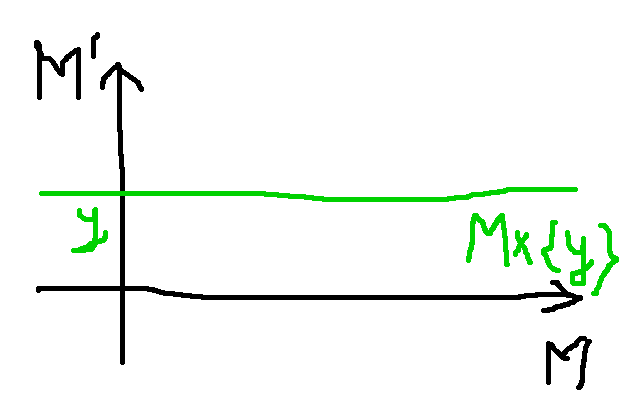
\includegraphics[width=0.4\textwidth]{at2.png}
        \end{center}
        
        \item Let $M, M^{\prime}$ be metric spaces. Consider the projection functions
        \[
            \pi: M \oplus_p M^{\prime} \rightarrow M,\left(x, x^{\prime}\right) \mapsto x \quad \text{and}\quad \pi^{\prime}: M \oplus_p M^{\prime} \rightarrow M^{\prime},\left(x, x^{\prime}\right) \mapsto x^{\prime}
        \]
        For $\mathbf{x}=\left(x, x^{\prime}\right)$ and $\mathbf{y}=\left(y, y^{\prime}\right)$ in $M \oplus_p M^{\prime}$, we have
        \[
        d(\pi(\mathbf{x}), \pi(\mathbf{y}))=d(x, y) \leqslant \max \left\{d(x, y), d^{\prime}\left(x^{\prime}, y^{\prime}\right)\right\}=d_{\infty}(\mathbf{x}, \mathbf{y}) \leqslant d_p(\mathbf{x}, \mathbf{y})
        \]
        and so $\pi$ is 1-Lipschitz. The same holds for $\pi^{\prime}$.

        E.g., $\mathbb{C}^n \rightarrow \mathbb{C},\left(z_1, \ldots, z_n\right) \mapsto z_k$ is continuous. We deduce that polynomials in any number of variables are also continuous.
    \end{enumerate}
\end{example}

\subsection{Generalised triangle inequality}
Suppose \( u,x,y,z \in M \).
Then, \( \abs{d(u,x) - d(y,z)} \leq d(u,y) + d(x,z) \).
First,
\[
	d(u,x) \leq d(u,y) + d(y,x) \leq d(u,y) + d(y,z) + d(z,x)
\]
Rearranging,
\[
	d(u,x)-d(y,z) \leq d(u,y) + d(x,z)
\]
To achieve the negative, satisfying both conditions in the absolute value term,
\[
	d(y,z) \leq d(y,u) + d(u,x) + d(x,z)
\]
which gives
\[
	d(y,z) - d(u,x) \leq d(u,y) + d(x,z)
\]
as required.

\section{Topology of metric spaces}
\subsection{Open balls}
In a metric space, continuity at a point $x$ or convergence of a sequence to a point $x$ depends on the set of points close to $x$. This motivates the following.
\begin{definition}
	Let $(M, d)$ be a metric space and $x \in M$. We define the \textbf{open ball} in $M$ with centre $x$ and radius $r$ (or the open $r$-ball around $x$ ) as the set
    \[
    D_r(x)=\{y \in M: d(y, x)<r\}
    \]
    We sometimes write $D_r^M(x)$ to indicate the underlying metric space $M$.
\end{definition}
The open ball notation is a convenient syntax for denoting closeness in some metric space.
Note that
\[
    \begin{aligned}
        &x_n \rightarrow x \text { in } M \Longleftrightarrow \forall \varepsilon>0\quad \exists N \in \mathbb{N}\quad \forall n \geqslant N \quad x_n \in D_{\varepsilon}(x) \\
        &f: M \rightarrow M^{\prime} \text { is continuous at } x \Longleftrightarrow \forall \varepsilon>0\quad \exists \delta>0\quad f\left(D_\delta(x)\right) \subset D_{\varepsilon}(f(x))
    \end{aligned}
\]
\begin{definition}
	The closed ball of centre \( x \) and radius \( r \geq 0 \) is the set
	\[
		B_r(x) = \qty{y \in M \colon d(y,x) \leq r}
	\]
\end{definition}
\begin{example} 
	\begin{enumerate}
        \item \( \mathbb R \), \( D_r(x) = (x-r,x+r) \),
        \( B_r(x) = [x-r,x+r] \).
        \item \( (\mathbb R^2, d_p) \), $\displaystyle B_1(0) = \left\{ x \in \mathbb R^2 \colon \norm{x}_p \leq 1  \right\}$. 
        \item In $\mathbb{C}, D_r(x)$ and $B_r(x)$ are the open and closed discs with centre $x$ and radius $r$.
        \item Let \( M \) be a discrete metric space.
        Then for \( x \in M \),
        \[
            D_1(x) = \qty{x};\quad B_1(x) = M
        \]
    \end{enumerate}
\end{example}
\begin{note}
	\begin{enumerate}
        \item $D_r(x) \subset B_r(x) \subset D_s(x)$ whenever $r<s$.
        \item $d(x, y)=\min \left\{r \geqslant 0: y \in B_r(x)\right\}=\inf \left\{r>0: y \in D_r(x)\right\}$
    \end{enumerate}
\end{note}

\subsection{Neighbourhoods and openness}\ \vspace{-1.5em}
\begin{definition}
	Let \( M \) be a metric space, and \( U \subset M \).
	Then for \( x \in M \), we say that \( U \) is a \textbf{neighbourhood} of \( x \) (in \( M \)) if
	\[
		\exists r > 0\quad D_r(x) \subset U \iff \exists r > 0\quad B_r(x) \subset U
	\]
\end{definition}
\begin{definition}
	We say \( U \subset M \) is \textbf{open} in \( M \), or that \( U \) is an \textbf{open subset} of \( M \), if
	\[
		\forall x \in U\quad \exists r > 0\quad D_r(x) \subset U
	\]
	So \( U \) is a neighbourhood of all points in \( U \).
\end{definition}
\begin{example}
	\( D_r(x), B_r(x) \) are neighbourhoods of \( x \).
\end{example}
\begin{example}
	Let \( H = \qty{ z \in \mathbb C \colon \Im z \geq 0 } \).
	Let \( w \in H \) and \( \delta = \Im w \).
	If \( \delta > 0 \), then \( D_\delta(w) \subset H \).
	If \( \delta = 0 \), then for any \( r \), \( D_\delta(w) \not\subset H \).
	So \( H \) is not open.
\end{example}
\begin{lemma}
	Open balls are open.
\end{lemma}
\begin{proof}
	Let \( D_r(x) \) be an open ball in a metric space \( M \).
	We need to show that
	\[
		\forall y \in D_r(x)\quad \exists \delta > 0\quad D_\delta(y) \subset D_r(x)
	\]
	So let \( y \in D_r(x) \) and set \( \delta = r - d(x,y) \).
	Note that \( d(x,y) > 0 \), and by the triangle inequality,
	\[
		d(z,x) \leq d(z,y) + d(y,x) < \delta + (r-\delta) = r
	\]
	as required.
\end{proof}
\begin{corollary}
	Let \( M \) be a metric space, \( U \subset M \), \( x \in M \).
	Then \( U \) is a neighbourhood of \( x \) if and only if there exists an open subset \( V \) of \( M \) such that \( x \in V \subset U \).
\end{corollary}
\begin{proof}
	In the forward direction, there exists \( r > 0 \) such that \( D_r(x) \subset U \), so let \( V = D_r(x) \).
	Conversely, if \( V \) is open we can construct \( r > 0 \) such that \( D_r(x) \subset V \subset U \).
	So \( U \) is a neighbourhood of \( x \).
\end{proof}

\subsection{Continuity and convergence using topology}\ \vspace{-1.5em}
\begin{proposition}
	In a metric space \( M \), the following are equivalent.
	\begin{enumerate}[(i)]
		\item \( x_n \to x \);
		\item for all neighbourhoods \( U \) of \( x \) in \( M \), \( \exists N \in \mathbb N, \forall n \geq N, x_n \in U \);
		\item for all open neighbourhoods \( U \) of \( x \) in \( M \), \( \exists N \in \mathbb N, \forall n \geq N, x_n \in U \).
	\end{enumerate}
\end{proposition}
\begin{proof}
	((i) $ \Rightarrow$ (ii))
	Let \( U \) be a neighbourhood of \( x \).
	Then by definition \( \exists \varepsilon > 0, D_\varepsilon(x) \subset U \).
	Since \( x_n \to x \),
	\[
		\exists N \in \mathbb N, \forall n \geq N, x_n \in D_\varepsilon(x)
	\]
	hence \( \forall n \geq N, x_n \in U \).

	((ii) $ \Rightarrow$ (iii))
	This is clear since any open set \( U \) with \( x \in U \) is a neighbourhood of \( x \).

	((iii) $ \Rightarrow$ (i))
	Fix \( \varepsilon > 0 \).
	By the above lemma, \( U = D_\varepsilon(x) \) is open, and \( x \in U \).
	Then by (iii),
	\[
		\exists N \in \mathbb N, \forall n \geq n, x_n \in U
	\]
	hence \( d(x_n, x) < \varepsilon \).
\end{proof}
\begin{proposition}
	Let \( f \colon M \to M' \) be a function between metric spaces.
	\begin{enumerate}[(a)]
		\item The following are equivalent for all \( x \in M \).
		      \begin{enumerate}[(i)]
			      \item \( f \) is continuous at \( x \);
			      \item for all neighbourhoods \( V \) of \( f(x) \) in \( M' \), there exists a neighbourhood \( U \) of \( x \) in \( M \) such that \( f(U) \subset V \);
			      \item for all neighbourhoods \( V \) of \( f(x) \) in \( M' \), \( f^{-1}(V) \) is a neighbourhood of \( x \) in \( M \).
		      \end{enumerate}
		\item The following are equivalent.
		      \begin{enumerate}[(i)]
			      \item \( f \) is continuous;
			      \item \( f^{-1}(V) \) is open in \( M \) for all open subsets \( V \) of \( M' \). (The inverse image of open set is open.)
		      \end{enumerate}
	\end{enumerate}
\end{proposition}
\begin{proof}
    We begin with part (a). 
    
    We first recall that (i) is the following statement.
    \[
        \forall \varepsilon>0 \quad \exists \delta>0 \quad f\left(D_\delta(x)\right) \subset D_{\varepsilon}(f(x))
    \]

    ((i) $\Rightarrow$ (ii)) Given a neighbourhood $V$ of $f(x)$ in $M^{\prime}$, there is an $\varepsilon>0$ such that $D_{\varepsilon}(f(x)) \subset V$. Since $f$ is continuous at $x$, there is a $\delta>0$ such that $f\left(D_\delta(x)\right) \subset D_{\varepsilon}(f(x))$. Set $U=D_\delta(x)$. Then $U$ is a neighbourhood of $x$ in $M$ and $f(U) \subset D_{\varepsilon}(f(x)) \subset V$.

    ((ii) $\Rightarrow$ (iii)) Given a neighbourhood $V$ of $f(x)$ in $M^{\prime}$, by assumption (ii) there is a neighbourhood $U$ of $x$ in $M$ such that $f(U) \subset V$. By definition of neighbourhood, there is a $r>0$ such that $D_r(x) \subset U$. It follows that $D_r(x) \subset U \subset f^{-1}(V)$, and hence $f^{-1}(V)$ is a neighbourhood of $x$ in $M$.

    ((iii) $\Rightarrow$ (i)) Given $\varepsilon>0$, the set $V=D_{\varepsilon}(f(x))$ is a neighbourhood of $f(x)$ in $M^{\prime}$, and hence $f^{-1}(V)$ is a neighbourhood of $x$ in $M$ by assumption. By definition, there is a $\delta>0$ such that $D_\delta(x) \subset f^{-1}(V)$. It follows that $f\left(D_\delta(x)\right) \subset V=D_{\varepsilon}(f(x))$. 

    We now deduce part (b).

    ((i) $\Rightarrow$ (ii)) Let $V$ be an open set in $M^{\prime}$. Fix $x \in f^{-1}(V)$. Then $f(x) \in V$, and so $V$ is a neighbourhood of $f(x)$ in $M^{\prime}$. Since $f$ is continuous at $x$, it follows from (a) that $f^{-1}(V)$ is a neighbourhood of $x$ in $M$. This holds for any $x \in f^{-1}(V)$, and thus $f^{-1}(V)$ is open in $M$.

    ((ii) $\Rightarrow$ (i)) Let $x \in M$ and let $\varepsilon>0$. Since $V=D_{\varepsilon}(f(x))$ is open in $M^{\prime}$, it follows that $f^{-1}(V)$ is open in $M$ by assumption. Since $f(x) \in V$, we have $x \in f^{-1}(V)$. Thus, there is a $\delta>0$ such that $D_\delta(x) \subset f^{-1}(V)$. It follows that $f\left(D_\delta(x)\right) \subset V=D_{\varepsilon}(f(x))$. This shows that $f$ is continuous at every $x \in M$, and thus $f$ is continuous.
\end{proof}

\begin{definition}
	The \textbf{topology} of a metric space \( M \) is the family of all open subsets of \( M \).
\end{definition}
\begin{proposition}
	The topology of a metric space satisfies
	\begin{enumerate}[(i)]
		\item \( \varnothing \) and \( M \) are open;
		\item if \( U_i \) are open in \( M \) for \( i \in I \) (\( I \) may be countable or uncountable), then \( \bigcup_{i \in I} U_i \) is open in \( M \);
		\item if \( U, V \) are open then \( U \cap V \) is open.
	\end{enumerate}
\end{proposition}
\begin{proof}
	(ii): Let \( x \in \bigcup_{i \in I} U_i \), then \( \exists i_a \in I, x \in U_{i_a} \).
	Then since \( U_{i_a} \) is open, \( \exists \delta > 0, D_r(x) \subset U_{i_a} \subset \bigcup_{i \in I} U_i \)

	(iii) Given \( x \in U \cap V \), since \( U \) is open then \( \exists r > 0 \), \( D_r(x) \subset U \) and \( \exists s > 0 \), \( D_s(x) \subset V \).
	Then let \( t = \min(r,s) \), and \( D_t(x) = D_r(x) \cap D_s(x) \subset U \cap V \).
\end{proof}

\subsection{Properties of topology of metric space}\ \vspace{-1.5em}
\begin{definition}
	Let $M$ be a metric space and $A \subset M$. We say $A$ is closed in $M$ (or that $A$ is a closed subset of $M)$ if for every sequence $\left(x_n\right)$ in $A$ that converges in $M$, we have $\lim _{n \rightarrow \infty} x_n$ is in $A$.
\end{definition}
\begin{lemma}
	Closed balls are closed.
\end{lemma}
\begin{proof}
	Consider \( B_r(x) \) in \( M \).
	Consider further \( (x_n) \in B_r(x) \) such that \( x_n \to z \) in \( M \).
	\[
		d(z,x) \leq d(z,x_n) + d(x_n,x) \leq d(z,x_n) + r \to r
	\]
	Hence \( d(z,x) \leq r \), so \( z \in B_r(x) \).
\end{proof}
\begin{example}
	\begin{enumerate}
        \item \( [0,1] = B_{1/2}(1/2) \) is closed in \( \mathbb R \).
        This is not open, for instance consider \( D_r(0) \not\subset [0,1] \).
    
        \item \( (0,1) = D_{1/2}(1/2) \) is open in \( \mathbb R \).
        This is not closed, for instance the sequence \( \frac{1}{n+1} \to 0\) in \( \mathbb R \).
    
        \item \( \mathbb R \) and \( \varnothing \) are open and closed in \( \mathbb R \).
    
        \item \( (0,1] \) in \( \mathbb R \) is neither open nor closed.
        \( D_r(1) \not\subset (0,1] \) and \( \frac{1}{n} \to 0 \not\in (0,1] \).
    \end{enumerate}
\end{example}
\begin{lemma}
	Let \( A \subset M \).
	Then \( A \) is closed in \( M \) if and only if \( M \setminus A \) is open in \( M \).
\end{lemma}
\begin{proof}
	Let \( A \) be closed.
	Suppose \( M \setminus A \) is not open.
	Then \( \exists x \in M \setminus A, \forall r > 0, D_r(x) \not\subset M \setminus A \), so \( D_r(x) \cap A \neq \varnothing \).
	In particular, for every \( n \) we can choose a point in \( D_{1/n}(x) \cap A \).
	Then, \( d(x_n,x) < \frac{1}{n} \to 0 \) and \( x_n \in A \) which contradicts the fact that \( A \) is closed.

	Conversely, assume \( M \setminus A \) is open, but suppose \( A \) is not closed.
	Then there exists a sequence \( (x_n) \in A \) such that \( x_n \to x \) in \( M \) but \( x \not\in A \).
	Since \( x \in M \setminus A \) and \( M \setminus A \) is open, there exists \( \varepsilon > 0, D_\varepsilon(x) \subset M \setminus A \).
	Since \( x_n \to x \), we must have \( \exists N \in \mathbb N, \forall n \geq N, x_n \in D_\varepsilon(x) \) and hence \( x_n \in M \setminus A \), contradiction.
\end{proof}
\begin{example}
	Let \( M \) be a discrete metric space.
	Let \( A \subset M \).
	Then for all \( x \in A \), \( D_1(x) = \qty{x} \subset A \).
	Hence \( A \) is open.
	So in a discrete metric space, all subsets are open.
	Hence every subset is closed.
\end{example}

\subsection{Homeomorphisms}
Recall that a map $f: M \rightarrow M^{\prime}$ between metric spaces is an isometry if it is bijective and isometric $\left(d^{\prime}(f(x), f(y))=d(x, y)\right.$ for all $\left.x, y \in M\right)$. This is the correct notion of structure-preserving map for metric spaces provided we are interested in metric properties, i.e., properties that depend on the metric itself. What if we are only interested in the topology that comes from the metric?

\begin{definition}
	A map \( f \colon M \to M' \) between metric spaces is called a \textbf{homeomorphism} if \( f \) is a bijection and \( f, f^{-1} \) are continuous.

	Equivalently, \( f \) is a bijection, and for all open sets \( V \) in \( M' \), \( f^{-1}(V) \) is open in \( M \), and for all open sets \( U \) in \( M \), \( f(U) \) is open in \( M' \).

	If there exists a homeomorphism between \( M, M' \), we say that \( M, M' \) are \textbf{homeomorphic}.
\end{definition}
\begin{example}
	Consider \( (0,\infty) \) and \( (0,1) \).
	Consider the map \( x \mapsto \frac{1}{x+1} \) with inverse \( x \mapsto \frac{1}{x} - 1 \).
	These are continuous, so the metric spaces are homeomorphic.
\end{example}
\begin{remark}
\begin{enumerate}
    \item Every isometry is a homeomorphism. Converse is false.
    \item Isometric metric spaces are homeomorphic. Converse is false.
    \item The identity map on a metric space is a homeomorphism, the inverse of a homeomorphism is a homeomorphism and the composite of homeomorphisms is a homeomorphism. It follows that being homeomorphic is an equivalence relation.
    \item Let $f: M \rightarrow M^{\prime}$ be a homeomorphism. If $U$ is an open subset of $M$, then $f(U)=\left(f^{-1}\right)^{-1}(U)$ is open in $M^{\prime}$, and conversely, if $V$ is an open subset of $M^{\prime}$, then $f^{-1}(V)$ is open in $M$. So we have a bijection between the topologies of $M$ and $M^{\prime}$.
    \item Let $f: M \rightarrow M^{\prime}$ be a homeomorphism. Then $\left(x_n\right)$ is convergent in $M$ if and only if $\left(f\left(x_n\right)\right)$ is convergent in $M^{\prime}$. Also, $g: N \rightarrow M$ is continuous if and only if $f \circ g$ is continuous, and $h: N \rightarrow M^{\prime}$ is continuous if and only if $f^{-1} \circ h$ is continuous. Similar comment applies to functions from $M$ and $M^{\prime}$.
    \item A continuous bijection need not be a homeomorphism. E.g.,
    Id: $(\mathbb{R}$, discrete$) \rightarrow(\mathbb{R}$, euclidean$)$
\end{enumerate}
\end{remark}

\subsection{Equivalence of metrics}\ \vspace{-1.5em}
\begin{definition}
	Let \( d, d' \) be metrics on a set \( M \).
	We say that \( d, d' \) are \textbf{equivalent}, written \( d \sim d' \), if they define the same topology.
\end{definition}

\begin{remark}
	Remark Each of the following statements are equivalent to $d \sim d^{\prime}$.
\begin{enumerate}
    \item The identity map Id: $(M, d) \rightarrow\left(M, d^{\prime}\right)$ is a homeomorphism. Note that this is stronger than saying that $(M, d)$ and $\left(M, d^{\prime}\right)$ are homeomorphic.
    \item $(M, d)$ and $\left(M, d^{\prime}\right)$ have the same convergent sequences.
    \item For every metric space $N$ and every $f: N \rightarrow M, f$ is continuous with respect to $d$ if and only if it is continuous with respect to $d^{\prime}$.
    \item For every metric space $N$ and every $f: M \rightarrow N, f$ is continuous with respect to $d$ if and only it is continuous with respect to $d^{\prime}$.
\end{enumerate}
\end{remark}

\begin{definition}
	Let \( d, d' \) be metrics on \( M \).
	Then we say \( d, d' \) are \textbf{uniformly equivalent}, written \( d \sim_u d' \) if
	\[
		\mathrm{id} \colon (M, d) \to (M, d');\quad \mathrm{id} \colon (M, d') \to (M, d)
	\]
	are uniformly continuous.
	We say \( d, d' \) are \textbf{Lipschitz equivalent}, written \( d \sim_\mathrm{Lip} d' \), if the identity maps above are Lipschitz.
\end{definition}
Equivalently, \( d \sim_\mathrm{Lip} d' \) if \( \exists a > 0, b > 0, ad(x,y) \leq d'(x,y) \leq bd(x,y) \).
	Note, \( d \sim_\mathrm{Lip} d' \implies d \sim_u d' \implies d \sim d' \).
\begin{example}
	\begin{enumerate}
        \item Given \( (M,d) \), define \( d'(x,y) = \min(1,d(x,y)) \).
        This defines a metric on \( M \), and \( d' \sim_u d \).
    
        \item On \( M \times M' \), \( d_1, d_2, d_\infty \) are pairwise Lipschitz equivalent.
    
        \item Consider \( C[0,1] \).
        The \( L_1 \) metric and the uniform metric are not equivalent.
        Consider \( f_n(x) = x^n \).
        This is convergent to zero in the \( L_1 \) metric but is not convergent in the uniform metric.
    
        \item The discrete metric and Euclidean metric on \( \mathbb R \) are not equivalent.
        This is becaue in the discrete metric all sets are open, but in the Euclidean metric there are some non-open sets.
    \end{enumerate}
\end{example}

\section{Completeness}
\subsection{Cauchy sequences}
In \( \mathbb R, \mathbb C \), every Cauchy sequence is convergent.
We wish to generalise this notion to an arbitrary metric space.
Recall that a sequence \( (x_n) \) in \( \mathbb R \) or \( \mathbb C \) is bounded if there exists \( c \in \mathbb R^+ \) such that \( \forall n \in \mathbb N, \abs{x_n} \leq c \).
\begin{definition}
	A sequence \( (x_n) \) in a metric space \( M \) is said to be \textbf{Cauchy} if
	\[
		\forall \varepsilon > 0\quad \exists N \in \mathbb N\quad \forall m,n \geq N\quad d(x_m,x_n) < \varepsilon
	\]
	The sequence is bounded if
	\[
		\exists z \in M\quad \exists r > 0\quad \forall n \in \mathbb N\quad x_n \in B_r(z)
	\]
	This is equivalent to
	\[
		\forall z \in M\quad \exists r > 0\quad \forall n \in \mathbb N\quad x_n \in B_r(z)
	\]
	by considering the triangle inequality around the given \( z \) point.
	In particular, if the metric arises from a norm, \( (x_n) \) is bounded if and only if \( \norm{x_n} \) is bounded.
\end{definition}
\begin{lemma}
	$ \text { convergent } \Longrightarrow \text { Cauchy } \Longrightarrow \text { bounded } $
\end{lemma}

\begin{proof}
    Let $\left(x_n\right)$ be a sequence in a metric space $M$.

    For the first implication, assume that $\left(x_n\right)$ is convergent $M$ and let $x$ denote its limit. Given $\varepsilon>0$, there exists $N \in \mathbb{N}$ such that $d\left(x_n, x\right)<\varepsilon / 2$ for all $n \geqslant N$. Then for $m, n \geqslant N$ we have
    \[
    d\left(x_m, x_n\right) \leqslant d\left(x_m, x\right)+d\left(x, x_n\right)<\varepsilon
    \]
    Thus, $\left(x_n\right)$ is Cauchy.

    For the second implication, assume that $\left(x_n\right)$ is Cauchy. Then there exists $N \in \mathbb{N}$ such that $d\left(x_m, x_n\right) \leqslant 1$ for all $m, n \geqslant N$. It follows that $x_n \in B_1\left(x_N\right)$ for all $n \geqslant N$. Now let
    \[
    r=\max \left\{d\left(x_1, x_N\right), d\left(x_2, x_N\right), \ldots, d\left(x_{N-1}, x_N\right), 1\right\}
    \]
    Then $x_n \in B_r\left(x_N\right)$ for all $n \in \mathbb{N}$.
\end{proof}

\begin{remark}
\begin{enumerate}
    \item Bounded $\centernot\implies$ Cauchy E.g., $0,1,0,1,0,1 \ldots$ in $\mathbb{R}$
    \item Cauchy $\centernot\implies$ convergent E.g., $(1 / n)$ in $(0, \infty)$.
\end{enumerate}
\end{remark}

\subsection{Completeness}\ \vspace{-1.5em}
\begin{definition}
	A metric space \( M \) is called \textbf{complete} if every Cauchy sequence in \( M \) converges in \( M \).
\end{definition}
\begin{example}
	\( \mathbb R, \mathbb C \) are complete.
\end{example}
\begin{proposition}
    If $M$ and $M^{\prime}$ are complete metric spaces, then $M \oplus_p M^{\prime}$ is also complete for $p=1,2$ and $\infty$.
\end{proposition}
\begin{proof}
    Let $\left(a_n\right)$ be a Cauchy sequence in $M \oplus_p M^{\prime}$ where $a_n=\left(x_n, x_n^{\prime}\right)$ for $n \in \mathbb{N}$. Given $\varepsilon>0$, there exists $N \in \mathbb{N}$ such that $d_p\left(a_m, a_n\right)<\varepsilon$ for all $m, n \geqslant N$. It follows that
    \[
    d\left(x_m, x_n\right) \leqslant d_p\left(a_m, a_n\right)<\varepsilon \quad \forall m, n \geqslant N
    \]
    and hence $\left(x_n\right)$, and by a similar argument $\left(x_n^{\prime}\right)$, is Cauchy. Since $M$ and $M^{\prime}$ are complete, $x_n \rightarrow x$ and $x_n^{\prime} \rightarrow x^{\prime}$ for some $x \in M$ and $x^{\prime} \in M^{\prime}$. Finally, let $a=\left(x, x^{\prime}\right)$. Then
    \[
    d_p\left(a_n, a\right) \leqslant d\left(x_n, x\right)+d^{\prime}\left(x_n^{\prime}, x^{\prime}\right) \rightarrow 0 \quad \text { as } n \rightarrow \infty
    \]
    Thus, $\left(a_n\right)$ in convergent in $M \oplus_p M^{\prime}$.
\end{proof}
\begin{note}
    $\left(a_n\right)$ is Cauchy if and only if $\left(x_n\right)$ and $\left(x_n^{\prime}\right)$ are Cauchy.
\end{note}

\begin{corollary}
$\mathbb{R}^n$ and $\mathbb{C}^n$ are complete in the $\ell_p$-metric for $p=1,2$ and $\infty$. In particular, $n$-dimensional real or complex euclidean space is complete.
\end{corollary}

\subsection{Completeness of subspaces}\ \vspace{-1.5em}

\begin{theorem}
    Let $S$ be an arbitrary set. Then the space $\ell_{\infty}(S)$ is complete in the uniform metric $D$.
\end{theorem}
\begin{proof}
    Let $\left(f_n\right)$ be a Cauchy sequence in $\ell_{\infty}(S)$. Then given $\varepsilon>0$, there exists $N \in \mathbb{N}$ such that for all $m, n \geqslant N$, we have
    \[
        D\left(f_m, f_n\right)=\sup _{x \in S}\left|f_m(x)-f_n(x)\right|<\varepsilon \implies \forall x \in S \quad\left|f_m(x)-f_n(x)\right|<\varepsilon.
    \]
    Thus, $\left(f_n\right)$ is uniformly Cauchy, and hence converges uniformly to a scalar function $f$ on $S$. It follows that $f$ is bounded, i.e., $f \in \ell_{\infty}(S)$. Finally, since $f_n \rightarrow f$ uniformly on $S$, given $\varepsilon>0$, there exists $N \in \mathbb{N}$ such that for all $n \geqslant N$ we have
    \[
        \forall x \in S \quad\left|f_n(x)-f(x)\right|<\varepsilon \implies D\left(f_n, f\right)=\sup _{x \in S}\left|f_n(x)-f(x)\right| \leqslant \varepsilon.
    \]
    This shows that $f_n \rightarrow f$ in the uniform metric.
\end{proof}

\begin{proposition}
    Let $N$ be a subspace of a metric space $M$.
    \begin{enumerate}[(i)]
        \item If $N$ is complete, then $N$ is closed in $M$.
        \item If $M$ is complete and $N$ is closed in $M$, then $N$ is complete.
    \end{enumerate}In particular, in a complete metric space, a subspace is closed if and only if it is complete.
\end{proposition}
\begin{proof}
    (i) Given $\left(x_n\right)$ in $N$, assume $x_n \rightarrow x$ in $M$. Then $\left(x_n\right)$ is Cauchy in $M$ by Lemma 12 , and hence Cauchy in $N$. Since $N$ is complete, $x_n \rightarrow y$ for some $y$ in $N$, and hence $x_n \rightarrow y$ in $M$. By uniqueness of limit, $x=y$, and thus $x \in N$, as required.

    (ii) Let $\left(x_n\right)$ be a Cauchy sequence in $N$. Then $\left(x_n\right)$ is Cauchy in $M$, and hence $x_n \rightarrow x$ for some $x$ in $M$. Since $N$ is closed, $x$ belongs to $N$. It follows that $x_n \rightarrow x$ in $N$.
\end{proof}

\begin{definition}
    Definition Let $(M, d)$ be a metric space. We define
    \[
    C_b(M)=\left\{f \in \ell_{\infty}(M): f \text { is continuous}\right\}.
    \]
    So in the real case, we have
    \[
    C_b(M)=\{f: M \rightarrow \mathbb{R}: f \text { is bounded and continuous}\}.
    \]
\end{definition}

\begin{note}
    $C_b(M)$ is a subspace of $\ell_{\infty}(M)$ in the uniform metric $D$.
\end{note}

\begin{theorem}
    $C_b(M)$ is complete in the uniform metric for any metric space $M$.
\end{theorem}

\begin{proof}
    It is enough to show that $C_b(M)$ is closed in $\ell_{\infty}(M)$. Let $\left(f_n\right)$ be a sequence in $C_b(M)$, let $f \in \ell_{\infty}(M)$, and assume that $f_n \rightarrow f$. We need to show that $f \in C_b(M)$, i.e., that $f$ is continuous. 
    
    Fix $a \in M$ and $\varepsilon>0$. Since $f_n \rightarrow f$, we can choose a large $n \in \mathbb{N}$ such that
    \[
    D\left(f_n, f\right)=\sup _{x \in M}\left|f_n(x)-f(x)\right|<\varepsilon.
    \]
    Since $f_n$ is continuous at $a$, there exists $\delta>0$ such that
    \[
    \forall x \in M \quad d(x, a)<\delta \Longrightarrow\left|f_n(x)-f_n(a)\right|<\varepsilon.
    \]
    It follows that for any $x \in M$, if $d(x, a)<\delta$, then
    \[
    \begin{aligned}
    |f(x)-f(a)| & \leqslant\left|f(x)-f_n(x)\right|+\left|f_n(x)-f_n(a)\right|+\left|f_n(a)-f(a)\right| \\
    & \leqslant \varepsilon+\varepsilon+\varepsilon=3 \varepsilon.
    \end{aligned}
    \]
    This shows that $f$ is continuous at $a$, and hence continuous.
\end{proof}

\begin{corollary}
    For any closed, bounded interval $[a, b]$ in $\mathbb{R}$, the space $C[a, b]$ of continuous scalar functions on $[a, b]$ is complete in the uniform metric.
\end{corollary}

\begin{definition}
    Let $S$ be a set and $(N, e)$ be a metric space. Define
    \[
    \ell_{\infty}(S, N)=\{f: S \rightarrow N: f \text { is bounded}\}
    \]
    We say $f$ is bounded if: $\exists y \in N \quad \exists r>0 \quad \forall x \in S \quad f(x) \in B_r(y)$

    Now assume that $g: S \rightarrow N$ is another bounded function: there exist $z \in N$ and $s>0$ such that $g(x) \in B_s(z)$ for all $x \in S$. Then
    \[
    \forall x \in S \quad e(f(x), g(x)) \leqslant e(f(x), y)+e(y, z)+e(z, g(x)) \leqslant r+e(y, z)+s
    \]
    It follows that $\sup _{x \in S} e(f(x), g(x))$ exists and will be denoted by $D(f, g)$. It is routine to verify that $D$ is a metric on $\ell_{\infty}(S, N)$ called the \textbf{uniform metric}.

    Now assume further that $(M, d)$ is a metric space. Define
    \[
    C_b(M, N)=\{f: M \rightarrow N: f \text { is bounded and continuous}\}
    \]
    which is a subspace of $\ell_{\infty}(M, N)$.
\end{definition}

\begin{theorem}\label{thm:19}
    Let $S$ be a set, $(M, d)$ and $(N, e)$ be metric spaces, and assume $N$ is complete. Then
\begin{enumerate}[(i)]
    \item $\ell_{\infty}(S, N)$ is complete in the uniform metric.
    \item $C_b(M, N)$ is complete in the uniform metric.
\end{enumerate}
\end{theorem}

\begin{proof}
    (i) Let $\left(f_k\right)$ be a Cauchy sequence in $\ell_{\infty}(S, N)$. We first show that $\left(f_k\right)$ is pointwise convergent. 
    
    Fix $x \in S$ and $\varepsilon>0$, since $\left(f_k\right)$ is Cauchy, there exists $K \in \mathbb{N}$ such that $D\left(f_i, f_j\right)<\varepsilon$ for all $i, j \geqslant K$. It follows that
    \[
    e\left(f_i(x), f_j(x)\right) \leqslant D\left(f_i, f_j\right)<\varepsilon \quad \text { for all } i, j \geqslant K
    \]
    Hence $\left(f_k(x)\right)$ is Cauchy in $N$, and thus convergent in $N$, since $N$ is complete. We can now define $ f: S \rightarrow N \text { by } f(x)=\lim _{k \rightarrow \infty} f_k(x) $.

    We next show that $f$ is bounded. 
    
    Since $ (f_k)$ is Cauchy, $\left(f_k\right)$ is bounded in the metric space $\ell_{\infty}(S, N)$. So there exists $g \in \ell_{\infty}(S, N)$ and $r>0$ such that $f_k \in B_r(g)$ for all $k \in \mathbb{N}$. Since $g$ is bounded, there exists $y \in N$ and $s>0$ such that $g(x) \in B_s(y)$ for all $x \in S$. It follows that for any $x \in S$ and $k \in \mathbb{N}$, we have
    \[
    e\left(f_k(x), y\right) \leqslant e\left(f_k(x), g(x)\right)+e(g(x), y) \leqslant D\left(f_k, g\right)+s \leqslant r+s
    \]
    and thus $f_k(x) \in B_{r+s}(y)$. By Lemma 2.10, the set $B_{r+s}(y)$ is closed in $N$. It follows that $f(x)=\lim _{k \rightarrow \infty} f_k(x) \in B_{r+s}(y)$ for all $x \in S$, and so $f$ is bounded, i.e., $f \in \ell_{\infty}(S, N)$.

    It remains to show that $f_k \rightarrow f$ in the uniform metric in $\ell_{\infty}(S, N)$. 
    
    Let $\varepsilon>0$. Since $\left(f_k\right)$ is Cauchy, there exists $K \in \mathbb{N}$ such that $D\left(f_i, f_j\right)<\varepsilon$ for all $i, j \geqslant K$. Fix $x \in S$ and $i \geqslant K$. Then
    \[
    e\left(f_i(x), f_j(x)\right) \leqslant D\left(f_i, f_j\right)<\varepsilon \quad \text { for all } j \geqslant K
    \]
    Since $f_j(x) \rightarrow f(x)$, and since the metric $e$ is continuous, it follows that $e\left(f_i(x), f(x)\right) \leqslant \varepsilon$. Since this holds for any $x \in S$, we have $D\left(f_i, f\right) \leqslant \varepsilon$, and this is true for any $i \geqslant K$. This proves that $f_i \rightarrow f$ in the uniform metric $D$.
    
    (ii) Since $\ell_{\infty}(M, N)$ is complete, it suffices to prove that $C_b(M, N)$ is closed in $\ell_{\infty}(M, N)$. Let $\left(f_k\right)$ be a sequence in $C_b(M, N)$, let $f \in \ell_{\infty}(M, N)$, and assume that $f_k \rightarrow f$ in the uniform metric. We need to show that $f \in C_b(M, N)$, i.e., that $f$ is continuous.

    Fix $a \in M$ and $\varepsilon>0$. Since $f_k \rightarrow f$, we can choose a large $k \in \mathbb{N}$ such that
    \[
    D\left(f_k, f\right)=\sup _{x \in M} e\left(f_k(x), f(x)\right)<\varepsilon
    \]
    Since $f_k$ is continuous at $a$, there exists $\delta>0$ such that
    \[
    \forall x \in M \quad d(x, a)<\delta \Longrightarrow e\left(f_k(x), f_k(a)\right)<\varepsilon
    \]
    It follows that for any $x \in M$, if $d(x, a)<\delta$, then
    \[
    \begin{aligned}
    e(f(x), f(a)) & \leqslant e\left(f(x), f_k(x)\right)+e\left(f_k(x), f_k(a)\right)+e\left(f_k(a), f(a)\right) \\
    & \leqslant \varepsilon+\varepsilon+\varepsilon=3 \varepsilon
    \end{aligned}
    \]
    This shows that $f$ is continuous at $a$, and hence continuous.
\end{proof}

\section{Contraction mappings}
\subsection{Contraction mapping theorem}\ \vspace{-1.5em}
\begin{definition}
    A map $f: M \rightarrow M^{\prime}$ between metric spaces is called a contraction mapping if
\[
\exists \lambda<1 \quad \forall x, y \in M \quad d^{\prime}(f(x), f(y)) \leqslant \lambda d(x, y)
\]
\end{definition}
\begin{note}
    Equivalently, $f$ is $\lambda$-Lipschitz with $\lambda<1$. Thus, a contraction mapping is continuous.
\end{note}

\begin{theorem}[Contraction Mapping Theorem]
    Let $M$ be a non-empty, complete metric space and let $f: M \rightarrow M$ be a contraction mapping. Then $f$ has a unique fixed point, i.e. there is a unique $z \in M$ such that $f(z)=z$. 
\end{theorem}
\begin{proof}
    Fix $\lambda<1$ such that $d(f(x), f(y)) \leqslant \lambda d(x, y)$ for all $x, y \in M$.

    Uniqueness: Assume $f(z)=z$ and $f(w)=w$. Then
    \[
    d(z, w)=d(f(z), f(w)) \leqslant \lambda d(z, w)
    \]
    Since $\lambda<1$, it follows that $z=w$. 

    Existence: Fix an arbitrary $x_0 \in M$ and define $\left(x_n\right)_{n=1}^{\infty}$ recursively by $x_n=f\left(x_{n-1}\right)$. Thus, $x_n=f^n(x)$, $f$ applies $n$ times.

    Idea: if $z= f^{\infty}(x_0)$, then $f(z)=z$.

    For any $n \in \mathbb{N}$, we have
    \[
    d\left(x_n, x_{n+1}\right)=d\left(f\left(x_{n-1}\right), f\left(x_n\right)\right) \leqslant \lambda d\left(x_{n-1}, x_n\right) \leqslant \ldots \leqslant \lambda^n d\left(x_0, x_1\right).
    \]
    It follows that for any $m, n \in \mathbb{N}$ with $n \geqslant m$, we have
    \begin{align*}
        d\left(x_m, x_n\right) &\leqslant \sum_{k=m}^{n-1} d\left(x_k, x_{k+1}\right) \leqslant \sum_{k=m}^{n-1} \lambda^k d\left(x_0, x_1\right)\\ 
        &=\frac{\lambda^m-\lambda^n}{1-\lambda} d\left(x_0, x_1\right) \leqslant \frac{\lambda^m}{1-\lambda} d\left(x_0, x_1\right).
    \end{align*}
    Since $\frac{\lambda^m}{1-\lambda} \rightarrow 0$ as $m \rightarrow \infty$, given $\varepsilon>0$, there exists $N \in \mathbb{N}$ such that $\frac{\lambda^m}{1-\lambda} d\left(x_0, x_1\right)<\varepsilon$ for all $m \geqslant N$, and then by above $d\left(x_m, x_n\right)<\varepsilon$ whenever $n \geqslant m \geqslant N$. This show that $\left(x_n\right)$ is Cauchy. Since $M$ is complete, $x_n \rightarrow z$ for some $z \in M$.
    Since $f$ is continuous, $f\left(x_n\right) \rightarrow f(z)$ as $n \rightarrow \infty$. On the other hand, $f\left(x_n\right)=x_{n+1} \rightarrow z$, so $f(z)=z$.
\end{proof}

\begin{remark}
\begin{enumerate}
    \item The proof not only shows the existence of a fixed point, but also a way of approximating it. Letting $n \rightarrow \infty$ in the inequality for $d\left(x_m, x_n\right)$, we obtain
    \[
    d\left(x_m, z\right) \leqslant \frac{\lambda^m}{1-\lambda} d\left(x_0, x_1\right) \quad \text { for all } m \in \mathbb{N}.
    \]
    Thus, the convergence is exponentially fast.
    \item $f: \mathbb{R} \backslash\{0\} \rightarrow \mathbb{R} \backslash\{0\}, x \mapsto x / 2$ is a contraction $\left(\lambda=\frac{1}{2}\right)$ but has no fixed point.
    \item $f: \mathbb{R} \rightarrow \mathbb{R}, x \mapsto x+1$ is isometric $(\lambda=1)$ but has no fixed point.
    \item $f:[1, \infty) \rightarrow[1, \infty), x \mapsto x+\frac{1}{x}$ satisfies $|f(x)-f(y)|<|x-y|$ for all $x, y \in[1, \infty)$ but has no fixed point.
\end{enumerate}
\end{remark}

\subsection{An application: initial value problem}
Given $y_0 \in \mathbb{R}$, consider the initial value problem (IVP)
\[
f^{\prime}(t)=f\left(t^2\right), \quad f(0)=y_0.
\]
Using contraction mapping theorem, we can show that it has a unique solution given an interval. 
\begin{proposition}
    The IVP above has a unique solution on $\left[0, \frac{1}{2}\right]$. In other words, there is a unique differentiable function $f:\left[0, \frac{1}{2}\right] \rightarrow \mathbb{R}$ satisfying $f(0)=y_0$ and $f^{\prime}(t)=f\left(t^2\right)$ for all $t \in\left[0, \frac{1}{2}\right]$.
\end{proposition}
\begin{proof}
    We show this in four steps. 

    \textit{Step 1: construct $f$.} $ f$ is a solution of the IVP if and only if
        \[
        f \in C\left[0, \frac{1}{2}\right] \quad \text { and } \quad f(t)=y_0+\int_0^t f\left(s^2\right) \mathrm{d} s \quad \text {for all } t \in\left[0, \frac{1}{2}\right].
        \]

    \textit{Step 2: introduce a contraction mapping.} $ M=C\left[0, \frac{1}{2}\right]$ is a non-empty, complete metric space in the uniform metric $D$. Define $T: M \rightarrow M$ by
    \[
    T(g)(t)=y_0+\int_0^t g\left(s^2\right) d s \quad \text { for } t \in\left[0, \frac{1}{2}\right] \text { and } g \in M
    \]
    $T(g)(t)$ is well-defined since $s \mapsto g\left(s^2\right)$ is continuous. $T(g)$ is continuous, and indeed even differentiable by the FTC with $(T g)^{\prime}(t)=g\left(t^2\right)$ for all $t \in\left[0, \frac{1}{2}\right]$.
    Thus $T g \in M$.
    By Step $1, f$ is a solution of the IVP if and only if $f \in M$ and $T f=f$.

    \textit{Step 3: show that $T$ is a contraction mapping.} For $g, h \in M$ we estimate
    \begin{align*}
        |(T g)(t)-(T h)(t)|&=\left|\int_0^t g\left(s^2\right)-h\left(s^2\right) d s\right| \\ 
        &\leqslant t \sup _{s \in\left[0, \frac{1}{2}\right]}\left|g\left(s^2\right)-h\left(s^2\right)\right| \\ 
        &\leqslant \frac{1}{2} D(g, h).
    \end{align*}
    Taking sup over all $t \in\left[0, \frac{1}{2}\right]$, we get $D(T g, T h) \leqslant \frac{1}{2} D(g, h)$. Thus, $T$ is a contraction mapping on $M$.

    \textit{Step 4: apply CMT.} By the Contraction Mapping Theorem, $T$ has a unique fixed point, and thus by Step 2, the IVP has a unique solution.
\end{proof}

\begin{remark}
    The same proof shows that for any $\delta \in(0,1)$, there is a unique solution $f_\delta$ to the IVP on $[0, \delta]$. For $\delta<\mu<1$, we have $f_\mu\restriction_{[0, \delta]}=f_\delta$ by uniqueness. Hence there is a unique solution to the IVP on $[0,1)$.
\end{remark}

\subsection{A theorem of Lindel\"{o}f-Picard}\ \vspace{-1.5em}
\begin{theorem}[Lindel\"{o}f-Picard]\label{thm:21}
    We are given $n \in \mathbb{N}, a, b, R \in \mathbb{R}$ with $a<b$ and $R>0, \mathbf{y}_0 \in \mathbb{R}^n$ and a continuous function
    \[
    \varphi:[a, b] \times B_R\left(\mathbf{y}_0\right) \rightarrow \mathbb{R}^n.
    \]
    Assume that there exists $K>0$ such that
    \[
    \|\varphi(t, \mathbf x)-\varphi(t, \mathbf y)\| \leqslant K\|\mathbf x-\mathbf y\| \quad \text { for all } t \in[a, b],\ \mathbf x, \mathbf y \in B_R\left(\mathbf y_0\right).
    \]
    Then there exists $\varepsilon>0$ such that for any $t_0 \in[a, b]$, the IVP
    \[
    f^{\prime}(t)=\varphi(t, f(t)), \quad f(t_0)=\mathbf y_0
    \]
    has a unique solution on $[c, d]=\left[t_0-\varepsilon, t_0+\varepsilon\right] \cap[a, b]$. In other words, there is a unique differentiable function $f:[c, d] \rightarrow \mathbb{R}^n$ that solves the above IVP.
\end{theorem}
\begin{note}
    \begin{enumerate}
        \item The statement that $f:[c, d] \rightarrow \mathbb{R}^n$ solves the IVP includes implicitly the condition that $f$ takes values in $B_R\left(y_0\right)$ (otherwise the differential equation would not make sense).
        \item The assumption on $ \varphi $ is called a Lipschitz condition in the second variable.
    \end{enumerate}
\end{note}
\subsubsection*{Aside: Differentiation and integration for functions $ [c,d]\to \mathbb{R}^{n} $}
Given a function $f:[c, d] \rightarrow \mathbb{R}^n$, we let $f_k=\pi_k \circ f:[c, d] \rightarrow \mathbb{R}$, where $\pi_k: \mathbb{R}^n \rightarrow \mathbb{R}$ is the $k^{\text {th }}$ coordinate projection mapping $\left(y_1, \ldots, y_n\right) \mapsto y_k$ for $k=1, \ldots, n$. Thus, $f(t)=\left(f_1(t), \ldots, f_n(t)\right)$ for every $t \in[c, d]$.
Now, $f$ is differentiable if each $f_k$ is differentiable, and
\[
f^{\prime}(t)=\left(f_1^{\prime}(t), \ldots, f_n^{\prime}(t)\right) \quad \text { for every } t \in[c, d]
\]
Also, if $f$ is continuous, then each $f_k$ is continuous, and hence integrable on $[c, d]$. 

We can then define the integral of $f$ coordinate-wise: $\int_c^d f(t) \dd t$ is the element $\mathbf{v} \in \mathbb{R}^n$ with $k^{\text {th}}$ coordinate $v_k=\int_c^d f_k(t) \dd t$. Observe that
\[
\begin{aligned}
\|v\|^2 &=\sum_{k=1}^n v_k^2=\sum_{k=1}^n v_k \int_c^d f_k(t) \dd t=\int_c^d \sum_{k=1}^n v_k f_k(t) \dd t \\
&=\int_c^d v \cdot f(t) \dd t \leqslant \int_c^d\|v\|\|f(t)\| \dd t=\|v\| \int_c^d\|f(t)\| \dd t.
\end{aligned}
\]
So we proved that $\left\|\int_c^d f(t) \dd t\right\| \leqslant \int_c^d\|f(t)\| \dd t$.

\begin{proof}[Proof of theorem.]
    Close balls are closed, so $B_R\left(\mathbf y_0\right)$ is a closed subset of $\mathbb{R}^n$. So $\varphi$ is a continuous function on the closed and bounded subset $[a, b] \times B_R\left(\mathbf y_0\right)$ of $\mathbb{R}^{n+1}$, and hence it is bounded. 
    
    Set $C=\sup \left\{\|\varphi(t, x)\|: t \in[a, b], x \in B_R\left(\mathbf y_0\right)\right\}$ and then set $\varepsilon=\min \left(\frac{R}{C}, \frac{1}{2 K}\right)$. We are going to show that this $\varepsilon$ works.

    Given $t_0 \in[a, b]$, set $[c, d]=\left[t_0-\varepsilon, t_0+\varepsilon\right] \cap[a, b]$. We need to prove that there is a unique differentiable function $f:[c, d] \rightarrow \mathbb{R}^n$ such that $f\left(t_0\right)=\mathbf y_0$ and $f^{\prime}(t)=\varphi(t, f(t))$ for all $t \in[c, d]$

    Since $B_R\left(\mathbf{y}_0\right)$ is closed in $\mathbb{R}^n$, and since $\mathbb{R}^n$ is complete, it follows that $B_R\left(\mathbf y_0\right)$ is complete. By Theorem \ref{thm:19}, the space $M=C\left([c, d], B_R\left(\mathbf y_0\right)\right)$ is complete in the uniform metric $D$. Also, $M \neq \emptyset$.

    Next, note that $f$ is a solution of the IVP on $[c, d]$ if and only if
    \[
    f \in M \quad \text { and } \quad f(t)=\mathbf y_0+\int_{t_0}^t \varphi(s, f(s)) \dd s \quad \text { for all } t \in[c, d]
    \]
    This follows from the FTC applied coordinate-wise.

    We next define
    \[
        T: M \rightarrow M \quad \text{by} \quad T(g)(t)=\mathbf y_0+\int_{t_0}^t \varphi(s, g(s)) \dd s \quad \text{for } t \in[c, d].
    \]
    We need to check that $T$ is well defined. First, the definition of $T(g)(t)$ makes sense, since
    $s \mapsto \varphi(s, g(s))$ is continuous. Next, $T(g)$ is a continuous function $[c, d] \rightarrow \mathbb{R}^n$.
    Indeed, $T(g)$ is differentiable with $(T g)^{\prime}(t)=\varphi(t, g(t))$ by the FTC. Finally, $T(g)$ takes values in $B_R\left(\mathbf y_0\right)$ since
    \begin{align*}
        \left\|T(g)(t)-\mathbf y_0\right\|&=\left\|\int_{t_0}^t \varphi(s, g(s)) \dd s\right\| \\ 
        &\leqslant\left|t-t_0\right| \sup _{s \in[c, d]}\|\varphi(s, g(s))\| \leqslant \varepsilon C \leqslant R \tag{$*$}
    \end{align*}
    for all $t \in[c, d]$. This shows that $T(g) \in M$.

    Now by the earlier observation, $f$ is a solution of the IVP if and only if $f \in M$ and $T f=f$. So the proof is complete if we can show that $T$ is a contraction mapping.

    Let $g, h \in M$. Note that by assumption,
    \[
    \|\varphi(s, g(s))-\varphi(s, h(s))\| \leqslant K\|g(s)-h(s)\| \leqslant K D(g, h) \quad \text {for all } s \in[c, d].
    \]
    It follows that for every $t \in[c, d]$ we have
    \begin{align*}
        \|(T g)(t)-(T h)(t)\| &=\left\|\int_{t_0}^t \varphi(s, g(s))-\varphi(s, h(s)) \mathrm{d} s\right\| \\
    & \leqslant\left|t-t_0\right| K D(g, h) \leqslant \varepsilon K D(g, h) \tag{$**$}
    \end{align*}
    Taking the sup over $t \in[c, d]$, we get $D(T g, T h) \leqslant \varepsilon K D(h, g) \leqslant \frac{1}{2} D(g, h)$. Thus, $T: M \rightarrow M$ is a contraction mapping, as required.
\end{proof}
\begin{remark}
    \begin{enumerate}
        \item In general, it is not possible to get a global solution, i.e., one on $[a, b]$.
        \item Inequalities $ (*),(* *) $ give rise to the choice of $ \epsilon $. 
        \item For any $\delta \in(0,1)$, taking $\varepsilon=\min \left(\frac{R}{c}, \frac{\delta}{K}\right)$ works. But by the uniqueness of the solution the choice does not matter for constructing the solution. So we can construct the solution for $\varepsilon=\min \left(\frac{R}{c}, \frac{1}{R}\right)$, on $\left(t_0-\varepsilon, t_0+\varepsilon\right) \cap[a, b]$.
    \end{enumerate}
\end{remark}

\subsection{A special case of Lindel\"of-Picard}
Theorem \ref{thm:21} handles $ n $th order ODEs as well. We do this next.

\begin{example}
    Let $a<b$ and $R>0$ be reals, let $\mathbf z=\left(z_0, z_1, \ldots, z_{n-1}\right) \in \mathbb{R}^n$ and let
\[
\psi:[a, b] \times B_R(\mathbf z) \rightarrow \mathbb{R}
\]
be a continuous function. Assume that for some $K>0$ we have
\[
|\psi(t, \bfx)-\psi(t, \bfy)| \leqslant K\|\bfx-\bfy\| \quad \text {for all } t \in[a, b] \text { and all } \bfx, \bfy \in B_R(\bfz) .
\]
Then there exists $\varepsilon>0$ such the for any $t_0 \in[a, b]$ the $n^{\text {th}}$-order IVP
\[
\begin{aligned}
g^{(n)}(t) &=\psi\left(t, g(t), g^{(1)}(t), g^{(2)}(t), \ldots, g^{(n-1)}(t)\right) \\
g^{(j)}\left(t_0\right) &=z_j \quad \text { for } 0 \leqslant j \leqslant n-1
\end{aligned}
\]
has a unique solution on $[c, d]=\left[t_0-\varepsilon, t_0+\varepsilon\right] \cap[a, b]$.
\end{example}

\begin{note}
    This means that there is a unique $n$-times differentiable function
    \[
    g:[c, d] \rightarrow \mathbb{R}
    \]
    that satisfies (1) for all $t \in[c, d]$. This implicitly includes the assumption that
    \[
    \left(g(t), g^{(1)}(t), g^{(2)}(t), \ldots, g^{(n-1)}(t)\right) \in B_R(\bfz)
    \]
    for all $t \in[c, d]$
\end{note}
\paragraph{Solution} Let us define $\varphi:[a, b] \times B_R(\bfz) \rightarrow \mathbb{R}^n$ by setting
\[
\varphi\left(t, x_0, x_1, \ldots, x_{n-1}\right)=\left(x_1, \ldots, x_{n-1}, \psi\left(t, x_0, x_1, \ldots, x_{n-1}\right)\right)
\]
for $t \in[a, b]$ and $\bfx=\left(x_0, x_1, \ldots, x_{n-1}\right) \in B_R(\bfz)$. Then $\varphi$ is continuous and satisfies 
\[
    \|\varphi(t, \bfx)-\varphi(t, \bfy)\| \leqslant(K+1)\|\bfx-\bfy\| \quad \text{for all } t \in[a, b] \text{ and all } \bfx, \bfy \in B_R(\bfz).
\]

By Lindelöf-Picard (Theorem \ref{thm:21}), there exists $\varepsilon>0$ such that the IVP
\[
    f^{\prime}(t)=\varphi(t, f(t)), \quad f\left(t_0\right)=\bfz
\]
has a unique solution on $[c, d]=\left[t_0-\varepsilon, t_0+\varepsilon\right] \cap[a, b]$. Let $f$ be this unique solution. 
Thus, $f:[c, d] \rightarrow B_R(\bfz)$ is a differentiable function with $f(t_0)=\bfz$ and $f^{\prime}(t)=\varphi(t, f(t))$ for all $t \in[c, d]$. 

Let $f_0, f_1, \ldots, f_{n-1}$ be the components of $f$, i.e., functions $f_j:[c, d] \rightarrow \mathbb{R}$ such that
\[
    f(t)=\left(f_0(t), f_1(t), \ldots, f_{n-1}(t)\right) \quad \text{for all } t \in[c, d].
\]
Since $f$ is a solution of the IVP, each $f_j$ is differentiable and
\begin{align*}
    &\left(f_0^{\prime}(t), f_1^{\prime}(t), \ldots, f_{n-1}^{\prime}(t)\right)=f^{\prime}(t)=\varphi(t, f(t)) \\
    &=\left(f_1(t), f_2(t), \ldots, f_{n-1}(t), \psi(t, f_0(t), f_1(t), \ldots, f_{n-1}(t)\right))\quad \text{for all }t\in [c,d].
\end{align*}
Set $g=f_0$. Comparing coordinates shows that $g$ is an $n$-times differentiable function $[c, d] \rightarrow \mathbb{R}$ with $g^{(j)}=f_j$ for $0 \leqslant j\le n-1$ (induction on $j$), and moreover
\begin{align*}
    g^{(n)}(t)=f_{n-1}^{\prime}(t)&=\psi\left(t, f_0(t), f_1(t), \ldots, f_{n-1}(t)\right) \\
&=\psi\left(t, g(t), g^{(1)}(t), \ldots, g^{(n-1)}(t)\right).
\end{align*}
for all $t \in[c, d]$. This solves the ODEs (first line of $g$).

Since $f\left(t_0\right)=\bfz$, we have $g^{(j)}\left(t_0\right)=f_j\left(t_0\right)=z_j$ for $0 \leqslant j \leqslant n-1$. This shows the initial conditions, and hence completes the proof of existence.

To prove uniqueness, assume that $\tilde{g}$ is another solution on $[c, d]$. Define $\tilde{f}:[c, d] \rightarrow B_R(\bfz)$ by setting $\tilde{f}(t)=\left(\tilde{g}(t), \tilde{g}^{(1)}(t), \ldots, \tilde{g}^{(n-1)}(t)\right)$. It is straightforward to verify that $\tilde{f}$ is a solution to the IVP of $f$. It follows that $\tilde{f}=f$ and $\tilde{g}=g$.

\end{document}